\documentclass{beamer}

\usepackage[utf8]{inputenc}
\usepackage{default}
\usepackage{amsmath}
\usepackage{color}
% \usepackage[dvipsnames]{xcolor}
% \usetheme{Dresden}
\usepackage{graphicx}
\usepackage[absolute,overlay]{textpos}
\usepackage{multicol}
\usepackage{cancel}

\definecolor{forestgreen}{rgb}{0.13,0.54,0.13}

\setbeamersize{text margin left=.5cm,text margin right=.5cm} 
\begin{document}

\title{Review of Synchrotron Radiation effects in the FFS}   
\author{Oscar Blanco}
\institute{CERN, LAL}
\date{\today} 

\definecolor{marron}{rgb}{0.64,0.16,0.16}

\newcommand{\LALlogo}{
  \setlength{\TPHorizModule}{1pt}
  \setlength{\TPVertModule}{1pt}
   % textblock{}{x,y}: pos(x) = leftUpperCorner + (x * \TPHorizModule), pos(y) = leftUpperCorner - (y * \TPVertModule)
%   \begin{textblock}{1}(5,205)
  \begin{textblock}{1}(5,220)
   
\includegraphics[height=1.6cm,keepaspectratio]{LAL.jpg}
  \end{textblock}
  }
\newcommand{\CLIClogo}{
  \setlength{\TPHorizModule}{1pt}
  \setlength{\TPVertModule}{1pt}
   % textblock{}{x,y}: pos(x) = leftUpperCorner + (x * \TPHorizModule), pos(y) = leftUpperCorner - (y * \TPVertModule)
  \begin{textblock}{1}(20,40)
   
\includegraphics[height=1.6cm,keepaspectratio]{CLIC.jpg}
  \end{textblock}
  }
% \newcommand{\LCWS}{
%   \setlength{\TPHorizModule}{1pt}
%   \setlength{\TPVertModule}{1pt}
%    % textblock{}{x,y}: pos(x) = leftUpperCorner + (x * \TPHorizModule), pos(y) = leftUpperCorner - (y * \TPVertModule)
%   \begin{textblock}{1}(5,35)
%    
\includegraphics[height=1.2cm,keepaspectratio]{LCWS12.jpg}
%   \end{textblock}
%   }
% \newcommand{\CLICWorkshop}{
%   \setlength{\TPHorizModule}{1pt}
%   \setlength{\TPVertModule}{1pt}
%    % textblock{}{x,y}: pos(x) = leftUpperCorner + (x * \TPHorizModule), pos(y) = leftUpperCorner - (y * \TPVertModule)
%   \begin{textblock}{1}(110,215)
%    
\includegraphics[height=0.8cm,keepaspectratio]{Workshop2013.jpg}
%   \end{textblock}
%   }


% \logo{%
%     
\includegraphics[width=1.4cm,height=1.4cm,keepaspectratio]{CERN.jpg}
% }
% \LALlogo
% \CLIClogo
% \CLICWorkshop
% \LCWS

\frame{\titlepage} 

\frame{\frametitle{Table of contents}\tableofcontents} 


\section{Beamsize}


% \begin{frame}{Beamsize}
% We are interested in the beamsize at the IP.
% \begin{multicols}{2}
% Horizontal plane
%  \begin{align*}
% \sigma^2 &= \sigma_0^2 + \sigma_g^2+\sigma_\delta^2 +{\color{red}\sigma_{rad}^2}\\
% \sigma^2 &= \sigma_0^2 + \sigma_g^2+\sigma_\delta^2 +\overbrace{{\color{blue}	\sigma_{rad}^2}}
% \end{align*}
% Vertical plane
%  \begin{align*}
% \sigma^2 &= \sigma_0^2 + \sigma_g^2+\sigma_\delta^2 +{\color{red}\sigma_{rad}^2}\\
% \sigma^2 &= \sigma_0^2 + \sigma_g^2+\sigma_\delta^2 +\overbrace{{\color{green}\sigma_{oide}^2}}
% \end{align*} 
% \end{multicols}
% \begin{align*}
%  \sigma_0 &\equiv \text{zero$^{\text{th}}$ order approx.}\\
%  \sigma_g &\equiv \text{result from geometric aberrations}\\
%  \sigma_\delta &\equiv \text{result from chromatic aberrations}\\
%  {\color{red}\sigma_{rad}} &\equiv \text{interaction with magnets}
% \end{align*}
% \end{frame}

\begin{frame}{Beamsize}
We are interested in the horizontal beamsize at the IP.
\begin{multicols}{1}
Horizontal plane
 \begin{align*}
%\sigma^2 &= \sigma_0^2 + \sigma_e^2 +{\color{red}\sigma_{rad}^2}\\
\sigma^2 &= \sigma_0^2 + \sigma_i^2 +{\color{blue}	\sigma_{rad}^2}
\end{align*}
% Vertical plane
%  \begin{align*}
% \sigma^2 &= \sigma_0^2 + \sigma_e^2 +{\color{red}\sigma_{rad}^2}\\
% \sigma^2 &= \sigma_0^2 + \sigma_e^2 +\overbrace{{\color{green}\sigma_{oide}^2}}
% \end{align*}
\end{multicols}
\begin{align*}
 \sigma_0 &\equiv \text{zero$^{\text{th}}$ order approx.}\\
 \sigma_i &\equiv \text{result from aberrations}\\
%  \sigma_\delta &\equiv \text{result from chromatic aberrations}\\
 {\color{blue}\sigma_{rad}} &\equiv \text{interaction with magnets}
\end{align*}
Evaluated by:
\begin{itemize}
 \item tracking of particles
 \item mathematical approximations
\end{itemize}
\end{frame}

% \section{Oide effect}
% \subsection{Introduction}
% \begin{frame}
%  \centering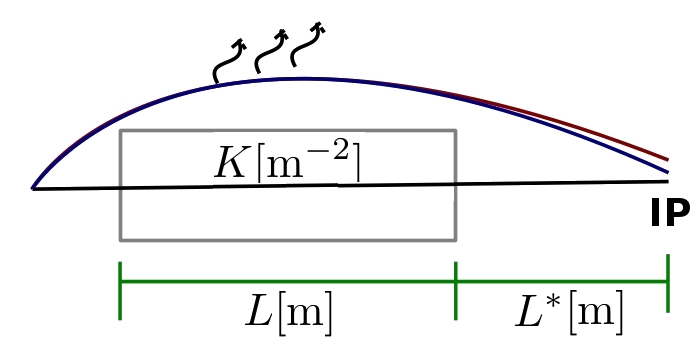
\includegraphics[width=8cm,height=4cm]{Oidea.jpg}
%  \begin{equation*}
% {\color{green} \sigma_{oide}^2} =\frac{110}{3\sqrt{6\pi}}r_e\lambda_e\gamma^5 {\color{forestgreen}F(\sqrt{K}L,\sqrt{K}L^*)}\left(\frac{\epsilon_y}{\beta^*_y}\right)^{5/2}
% \end{equation*}
% {\tiny
% \begin{equation*}
%  {\color{forestgreen}F(\sqrt{K}L,\sqrt{K}L^*)}=\int^{\sqrt{K}L}_0 |\sin\phi+\sqrt{K}L^*\cos\phi|^3\left[\int^\phi_0(\sin\phi'+\sqrt{K}L^*\cos\phi')^2d\phi'\right]^2d\phi
% \end{equation*}
% Equation derived by \cite{Oide}.
% }
% 
% \end{frame}
% \begin{frame}{Two approaches}
%  For a given $L^*$, what is the gradient K that minimizes ${\color{forestgreen}F(\sqrt{K}L,\sqrt{K}L^*)}$?
%  \begin{tabular}{ll}
%   %1) & 2) \\
%   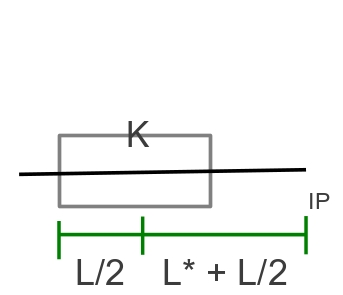
\includegraphics[width=4.5cm,height=3cm]{quad4.jpg} & 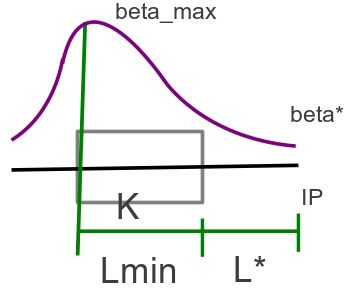
\includegraphics[width=4.5cm,height=3cm]{quad3.jpg}
%  \end{tabular}
% \begin{tabular}{l|c|c|c|}\cline{2-4}
% &$\beta_y^*$[mm] & $L^*$ [m] & $L$ [m]\\\hline
% CLIC 3TeV & 0.09 & 3.5 & 2.73\\\hline
% CLIC 500GeV & 0.40 & 4.3 & 3.35\\\hline
% ILC 500GeV & 0.48 & 3.5 &2.20\\\hline 
% \end{tabular}
% 
% \end{frame}
% \subsection{Results and conclusions}
% % \begin{frame}{Quad length}
% %  
% % \end{frame}
% \begin{frame}\hspace*{-1cm}
% 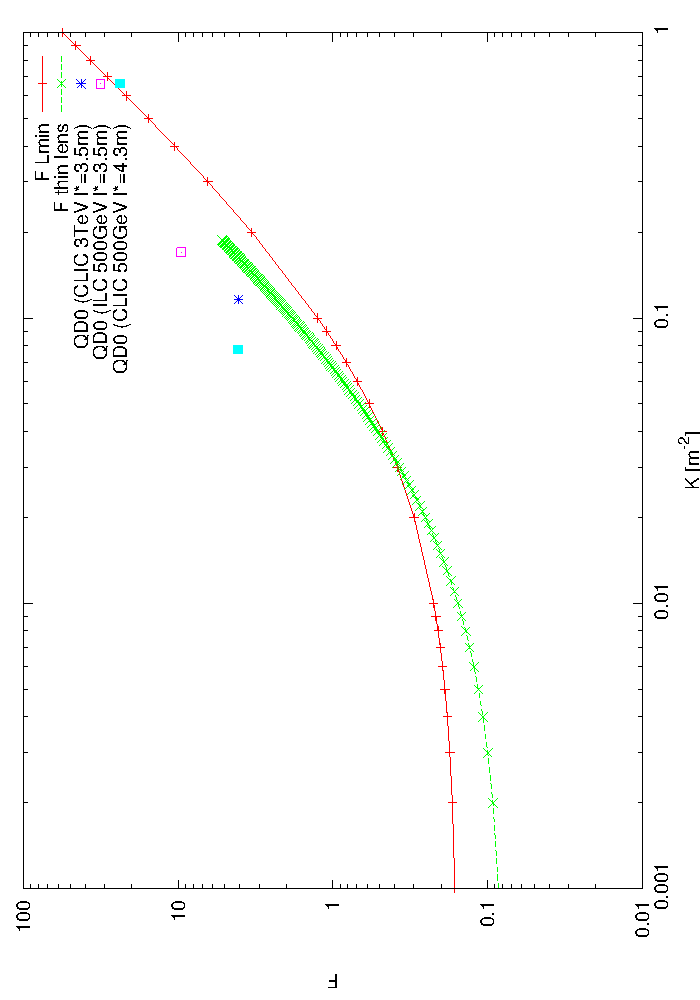
\includegraphics[width=6.7cm,height=13cm,angle=-90]{im10.png} 
% \begin{textblock}{1}(50,60)
% %    
\includegraphics[height=1.6cm,keepaspectratio]{LAL.jpg}
% \begin{tabular}{lc}
%  & ${\color{green}\sigma_{oide}}$[nm]\\
% CLIC 3TeV & 0.6387\\
% CLIC 500GeV & 0.0256\\
% ILC 500GeV & 0.0258\\
% \end{tabular}
% 
%   \end{textblock}
% \end{frame}
% 
% 
% % \subsection{Conclusions}
% \begin{frame}{Conclusions}
% \begin{itemize}
%  \item Longer quadrupoles for the final doublet with lower gradient could reduce the Oide effect.
%  \item There will always be a contribution to the beam size due to Oide effect.
%  \item Importance of this effect is increased when targeting the higher energies (CLIC 3TeV).
% \end{itemize}
% \end{frame}


\section{Radiation on bending magnets}
\subsection{Theoretical model}

\begin{frame}{Beam Radiation Model}

{\color{blue}$x$} describes the displacement of a particle at ($s=L$, e.g. IP) due to radiation, where
 all other effects are ignored.
 
 \begin{equation}
{\color{blue} x} = \sum_{i=1}^{N(T)}\Delta x_{i,total} - x_0
\end{equation}
\begin{itemize}
 \item $\Delta x_{i,total} $: is the total deviation due to the $i^{\text{th}}$ photon radiated
 \item $x_0$: is $\langle\sum_{i=1}^{N(T)}\Delta x_{i,total}\rangle$, \par \hspace*{1cm}in order to make $\langle {\color{blue}x}\rangle=0$,
 and ${\color{blue} \sigma_{rad}^2=\langle x^2\rangle}$
 \item $N$: is the number of photons radiated
 \item $T$: time to cross the bending magnet
\end{itemize}
\end{frame}
% 
% \begin{frame}{Finding $\Delta x_i$}
% $\Delta x_i$ is the effect at $(s=L)$ due to a photon of energy $u$ radiated at $s=s_i$, therefore it has to be propagated from $s_i$ to $L$.%\footnote{Sub-index $i$ has been dropped for clarity.}
% \begin{align}
%  \Delta x_i &= (u/E) R_{16}(s_i,L) 
% \end{align}
% 
% 
% According to Sands \cite{Sands}, $N\sim Poisson$, then
% \begin{equation}
%  \sigma_N^2 = \langle N\rangle ,\qquad x_0 = \langle N\rangle\langle \Delta x_{i,total}\rangle%,\qquad {\color{blue}\sigma_{rad}^2} = \langle N\rangle \langle \overline{\Delta x}^2\rangle
% \end{equation}
% \begin{align}
% \Delta x_{i,total} &= \frac{u}{E} \sqrt{\frac{\beta_L}{\beta}}\left[\eta\cos\Delta\phi_{s_i,L}+(\alpha\eta+\beta\eta')\sin\Delta\phi_{s_i,L}\right]\\
% &= \Delta x_i + \Delta x_{i,\eta} \qquad\footnotemark\notag
% \end{align}
% \addtocounter{footnote}{-1}
% \footnote{betatron oscillation + displacement}
% \end{frame}

\begin{frame}{Finding $\Delta x_i$}
$\Delta x_i$ is the effect at $(s=L)$ due to a photon of energy $u$ radiated at $s=s_i$, therefore it has to be propagated from $s_i$ to $L$.%\footnote{Sub-index $i$ has been dropped for clarity.}
\begin{align}
 \Delta x_i &= (u/E) R_{16}(s_i,L) 
\end{align}


It becomes:
{\small
\begin{equation*}
 {\color{blue}\sigma_{rad}^2}\approx C_2 \int \frac{E^5}{\rho^3}\left\{\sqrt{\frac{\beta_L}{\beta_s}}\left[\eta\cos\Delta\phi(s,L)+(\alpha\eta+\beta\eta')\sin\Delta\phi(s,L)\right]-\eta_L\right\}^2ds
\end{equation*}
}
\begin{itemize}
 \item $C_2=4.13\times10^{-11}[\text{m}^2\cdot\text{GeV}^{-5}]$
 \item $E$: is the beam energy
\end{itemize}
included in MAPCLASS2.\par

\end{frame}


% \begin{frame}{Finding $\Delta x_i$ (cont.)}
% We could do the following approximation,
% \begin{equation}
%  \langle\Delta x_{i,total}\rangle = \cancelto{0}{\langle\Delta x_i\rangle} + \langle \Delta x_{i,\eta}\rangle = (u/E) \eta_L
% \end{equation}
% when, $\eta_L=0$ it returns exactly the same result as Sands \cite{Sands}.\par
% when, $\eta_L \neq 0$ this is the term to be substracted from $\Delta x_{i,total}$ in order to obtain the correct contribution to radiation.\par
% \begin{equation}
% {\color{blue} x} = \sum_{i=1}^{N(T)}(\Delta x_{i,total} - \langle \Delta x_{i,total}\rangle)
% \end{equation}
% 
% \textbf{Now we have an approximation when $\eta_L\neq 0$.}
% \end{frame}

\newsavebox\radequ
\begin{lrbox}{\radequ}%
  \begin{minipage}{1.0\textwidth}%
  {\scriptsize%
 \raggedleft%
 \vspace*{-3.4cm}
    \begin{align*}
    {\color{blue}\sigma_{rad}^2} &= C_2\int_0^L \frac{E^5}{\rho^3}R_{16}^2(s,L)ds\\
    &= C_2\int_0^\theta \frac{E^5}{\rho^3}[\rho(1-\cos(\theta-\chi))]^2\rho d\chi\\
    &={\color{marron}C_2E^5\left[\frac{1}{4}(6\theta-8\sin\theta+\sin(2\theta))\right]\qquad\footnotemark}\\
    &={\color{marron}C_2E^5\left(\frac{\theta^5}{20}-\frac{\theta^7}{168}+\frac{\theta^9}{2880}-\frac{17\theta^{11}}{1330560}+O(\theta^{13})\right)}
     \end{align*} 
    }
  \end{minipage}
\end{lrbox}

% \begin{frame}{Result (from approximation)}
% 
% The contribution to beamsize due to radiation now can be calculated as:
% {\small
% \begin{equation*}
%  {\color{blue}\sigma_{rad}^2}\approx C_2 \int \frac{E^5}{\rho^3}\left\{\sqrt{\frac{\beta_L}{\beta_s}}\left[\eta\cos\Delta\phi(s,L)+(\alpha\eta+\beta\eta')\sin\Delta\phi(s,L)\right]-\eta_L\right\}^2ds
% \end{equation*}
% }
% \begin{itemize}
%  \item $C_2=4.13\times10^{-11}[\text{m}^2\cdot\text{GeV}^{-5}]$
%  \item $E$: is the beam energy
% \end{itemize}
% This expression was included in MAPCLASS2.\par
% It is possible to obtain a mathematical expression for one sbend magnet.
% \end{frame}

\subsection{One dipole}
\begin{frame}{One dipole (theoretical expression)}
Using $R_{16}= \rho(1-\cos\theta)$
\begin{tabular}{p{2cm}p{10cm}}
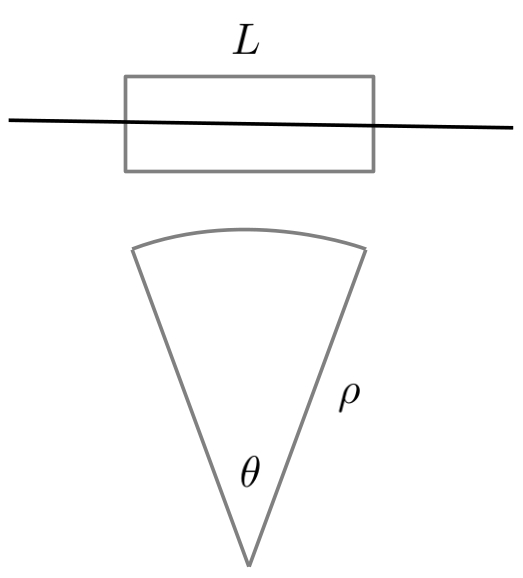
\includegraphics[width=4cm,height=4cm]{Bend.jpg}&\usebox{\radequ}%
\end{tabular}
{\scriptsize
Theoretical expression for a drift has been also derived.
Now, the {\color{marron}theoretical expression}, {\color{green}the approximated result} and {\color{red}tracking with PLACET} could be compared.\par
 Some care should be taken when using {\color{marron}the expression above} due to numerical precision.\par
 MAPCLASS2 uses on MAD-X twiss table results.\par
 PLACET has two different radiation methods ``Default'' and ``six\_dim''.\par
  Radiation beamsize has been normalized to the 
 {\color{marron}theoretical value}. \par
\addtocounter{footnote}{-1}
\footnote{If $E$ is considered constant.}
}

\end{frame}
\begin{frame}%{Results}
 \hspace*{2.3cm}Default Synrad\hspace*{3.3cm}Flag ``-six\_dim 1''\par
 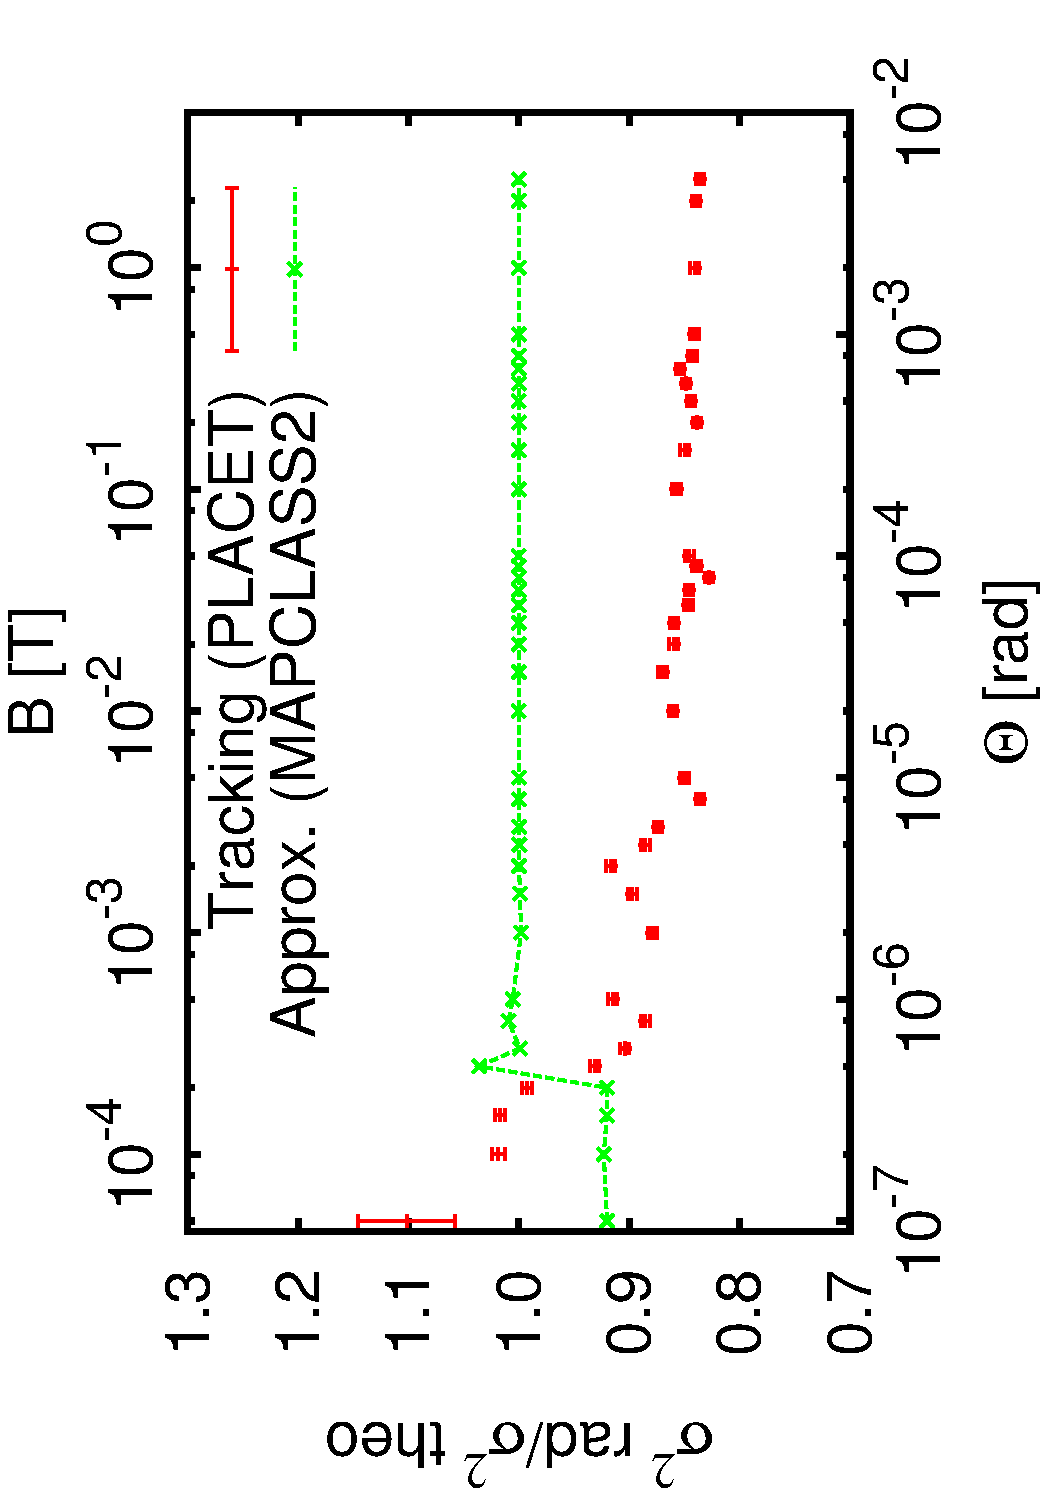
\includegraphics[scale=0.24,angle=-90]{sigma_angle.pdf}
 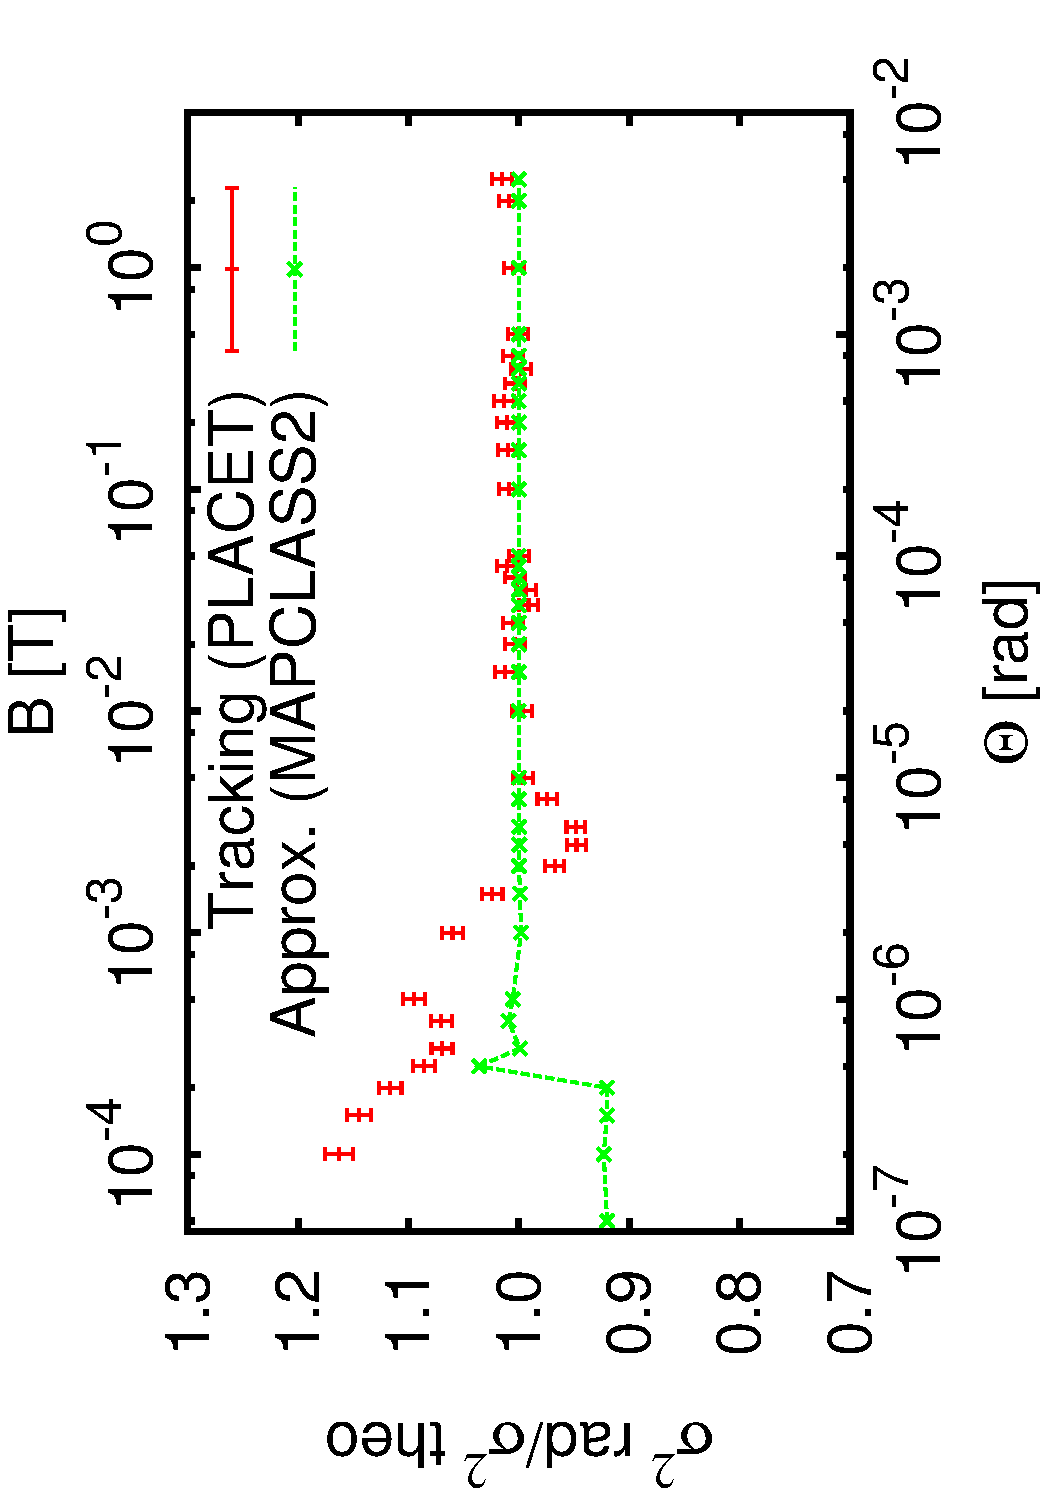
\includegraphics[scale=0.24,angle=-90]{sigma_angle_r06.pdf}\par
  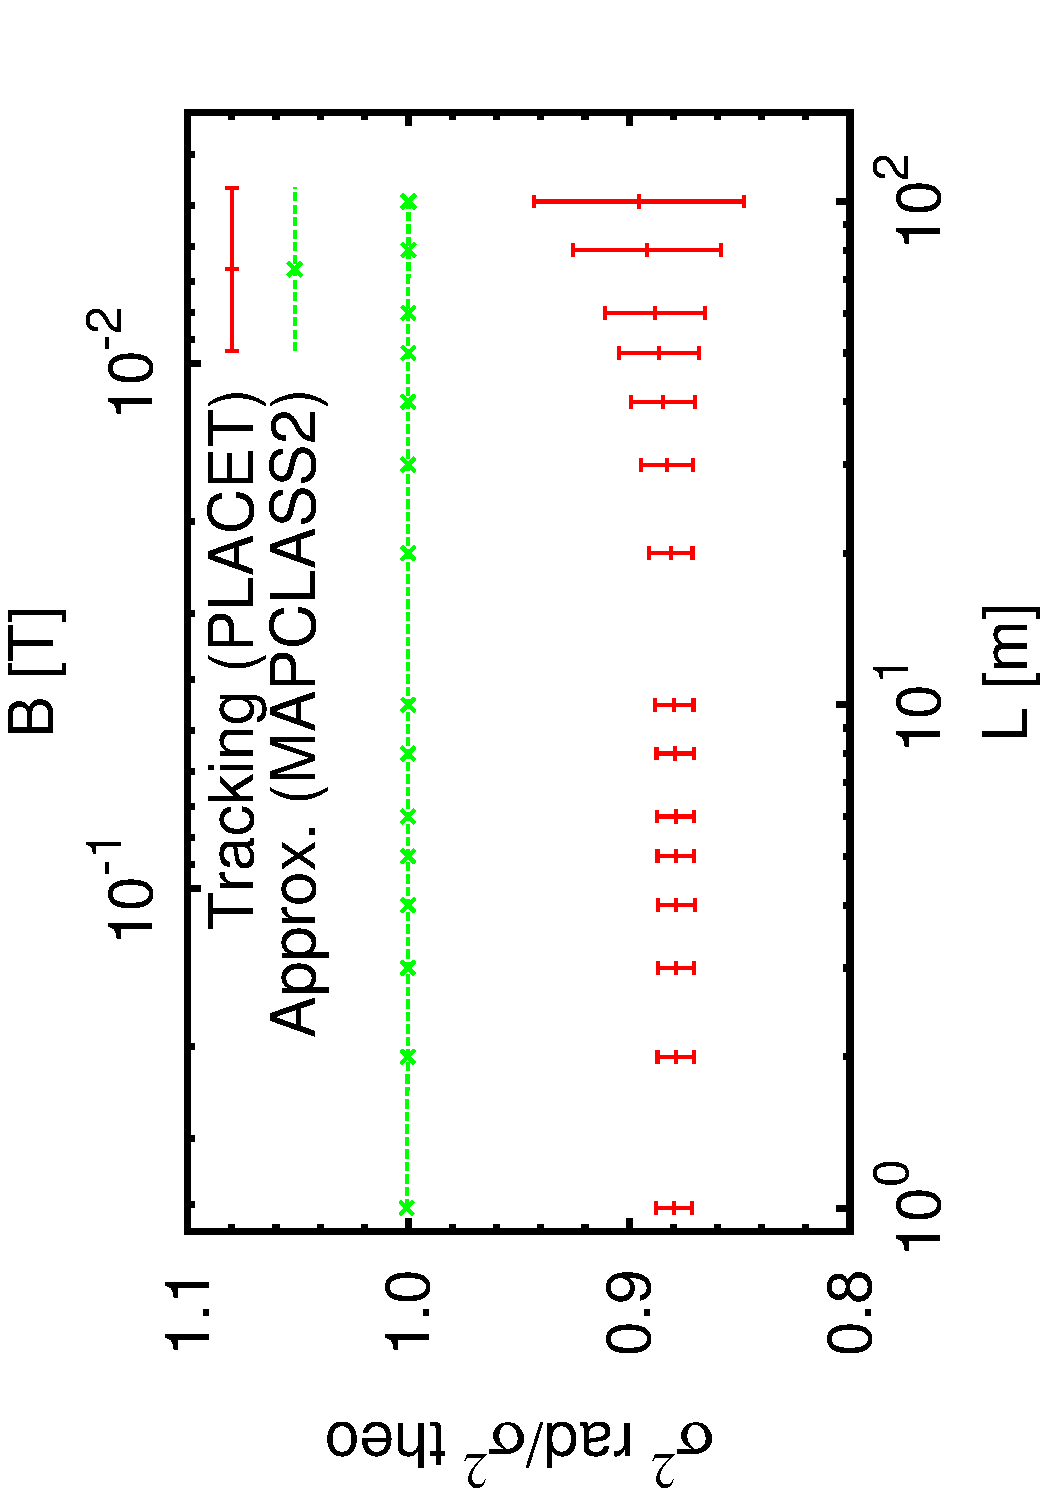
\includegraphics[scale=0.24,angle=-90]{sigma_Lbend.pdf}
 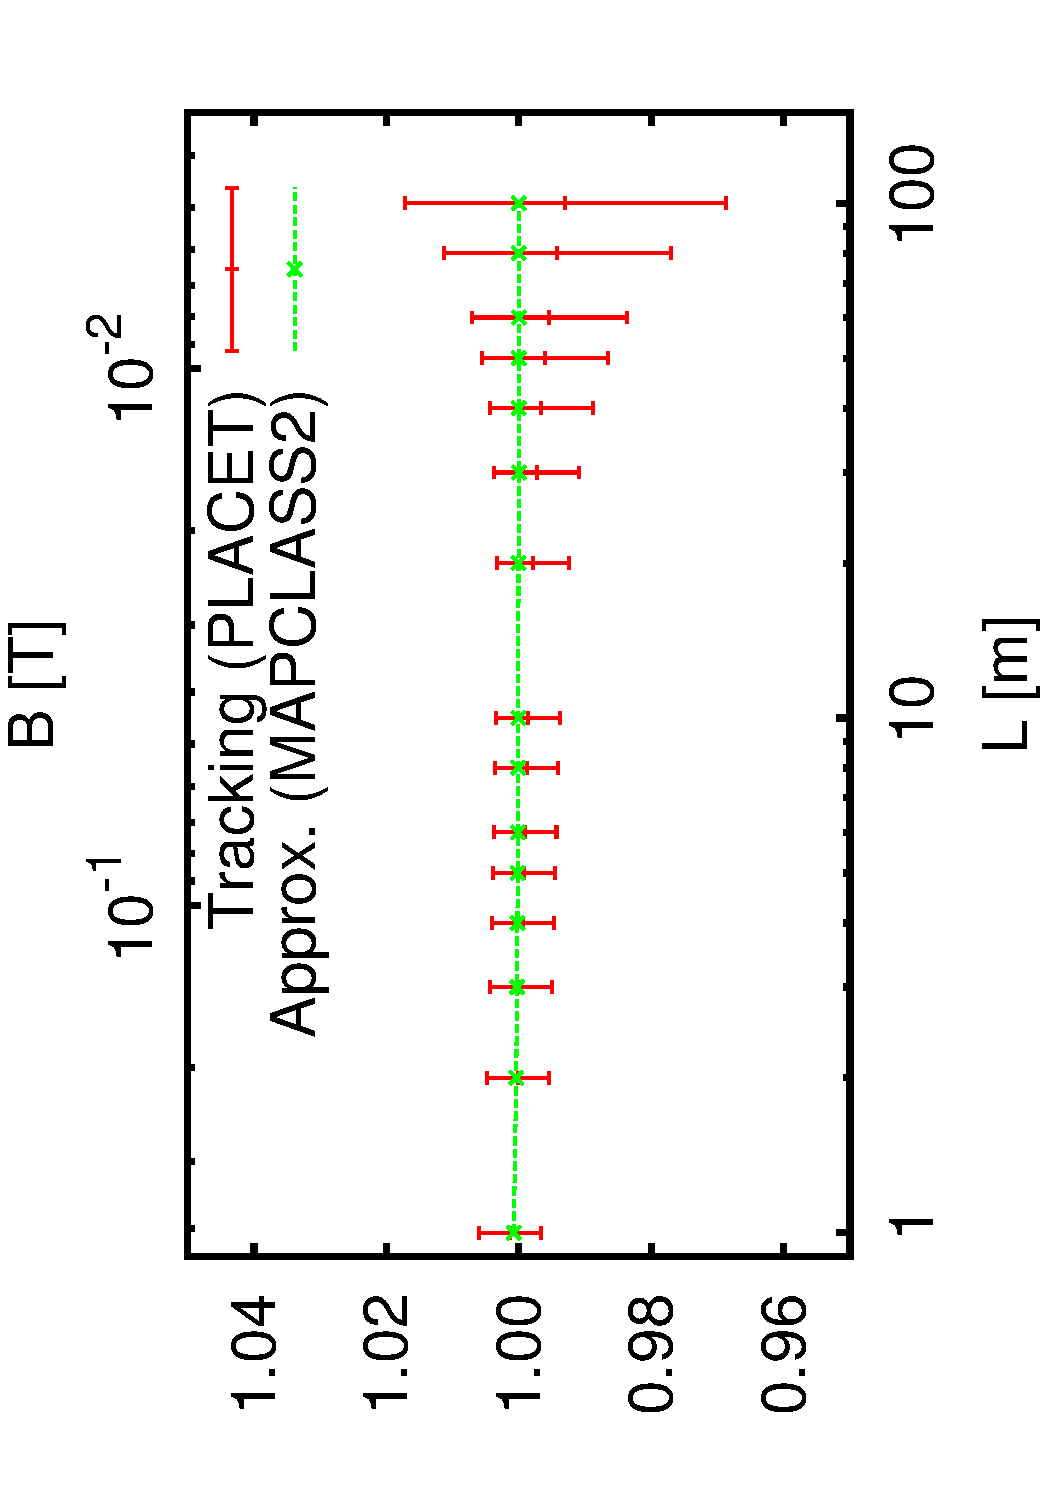
\includegraphics[scale=0.24,angle=-90]{sigma_Lbend_r6.pdf}\par

\end{frame}

\begin{frame}
  \hspace*{2.3cm}Default Synrad\hspace*{3.3cm}Flag ``-six\_dim 1''\par
 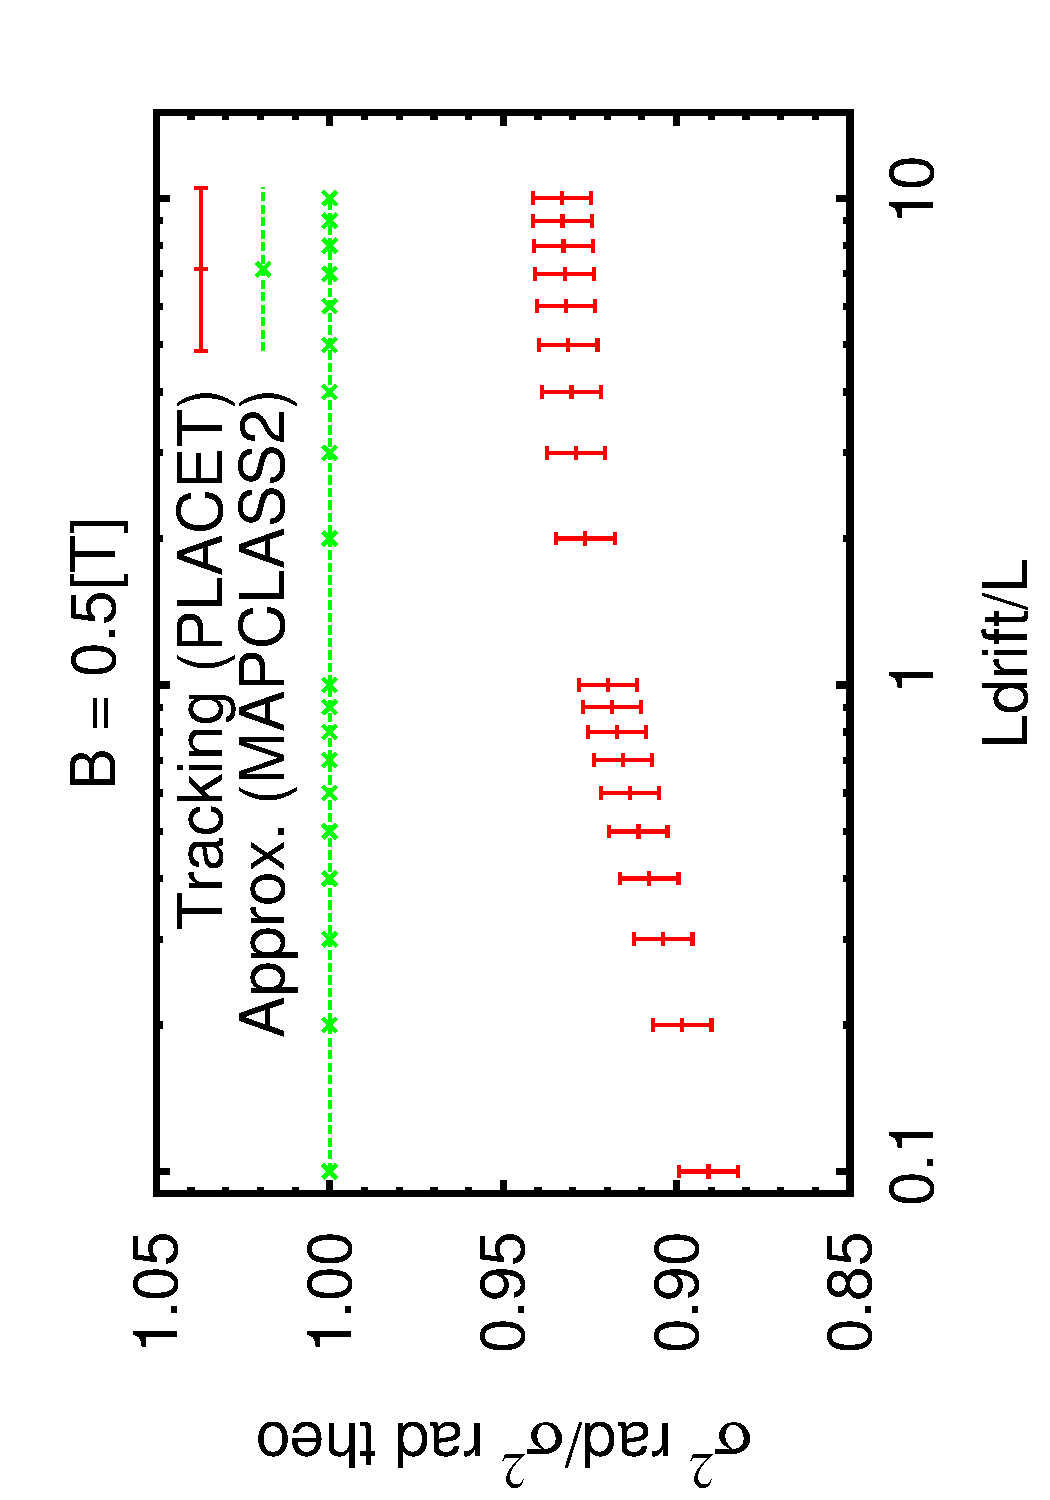
\includegraphics[scale=0.24,angle=-90]{sigma_Ldrift.pdf}
 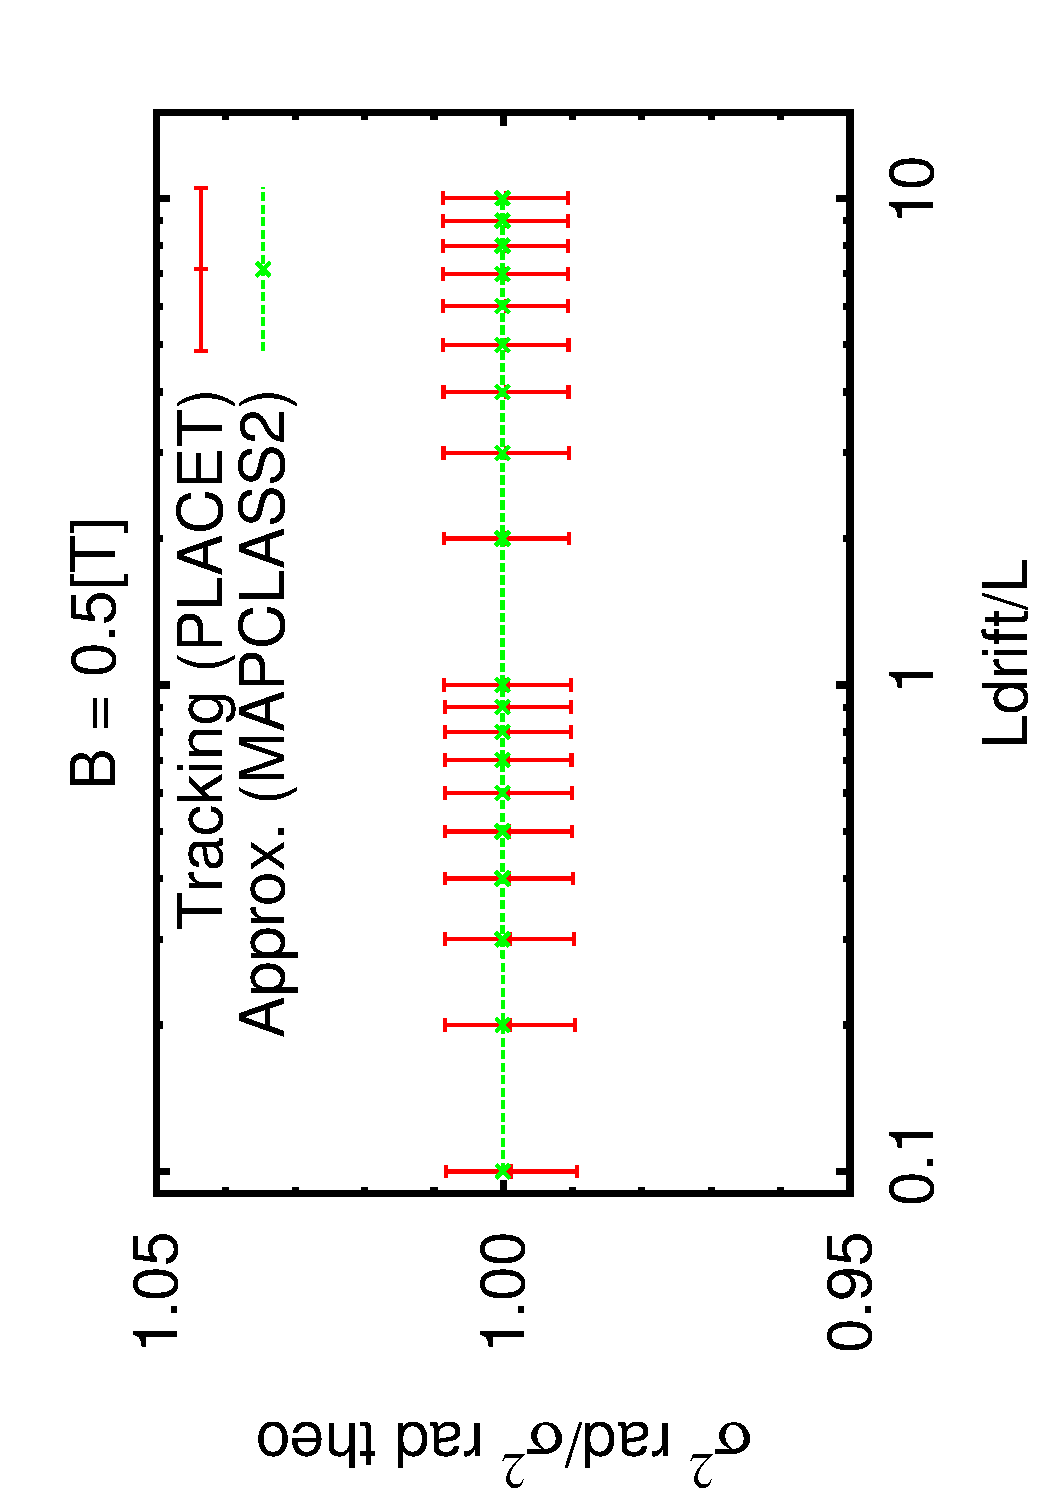
\includegraphics[scale=0.24,angle=-90]{sigma_Ldrift_r6.pdf}
\end{frame}

\newcommand{\twisslogo}{
  \setlength{\TPHorizModule}{1pt}
  \setlength{\TPVertModule}{1pt}
   % textblock{}{x,y}: pos(x) = leftUpperCorner + (x * \TPHorizModule), pos(y) = leftUpperCorner - (y * \TPVertModule)
%   \begin{textblock}{1}(5,205)
  \begin{textblock}{1}(200,80)
   Twiss
  \end{textblock}
  }

  \newcommand{\ptctwisslogo}{
  \setlength{\TPHorizModule}{1pt}
  \setlength{\TPVertModule}{1pt}
   % textblock{}{x,y}: pos(x) = leftUpperCorner + (x * \TPHorizModule), pos(y) = leftUpperCorner - (y * \TPVertModule)
%   \begin{textblock}{1}(5,205)
  \begin{textblock}{1}(200,190)
   ptc\_twiss
  \end{textblock}
  }
  
\begin{frame}
%    \hspace*{2.3cm}Twiss\hspace*{3.3cm}Flag ``ptc\_twiss''\par
 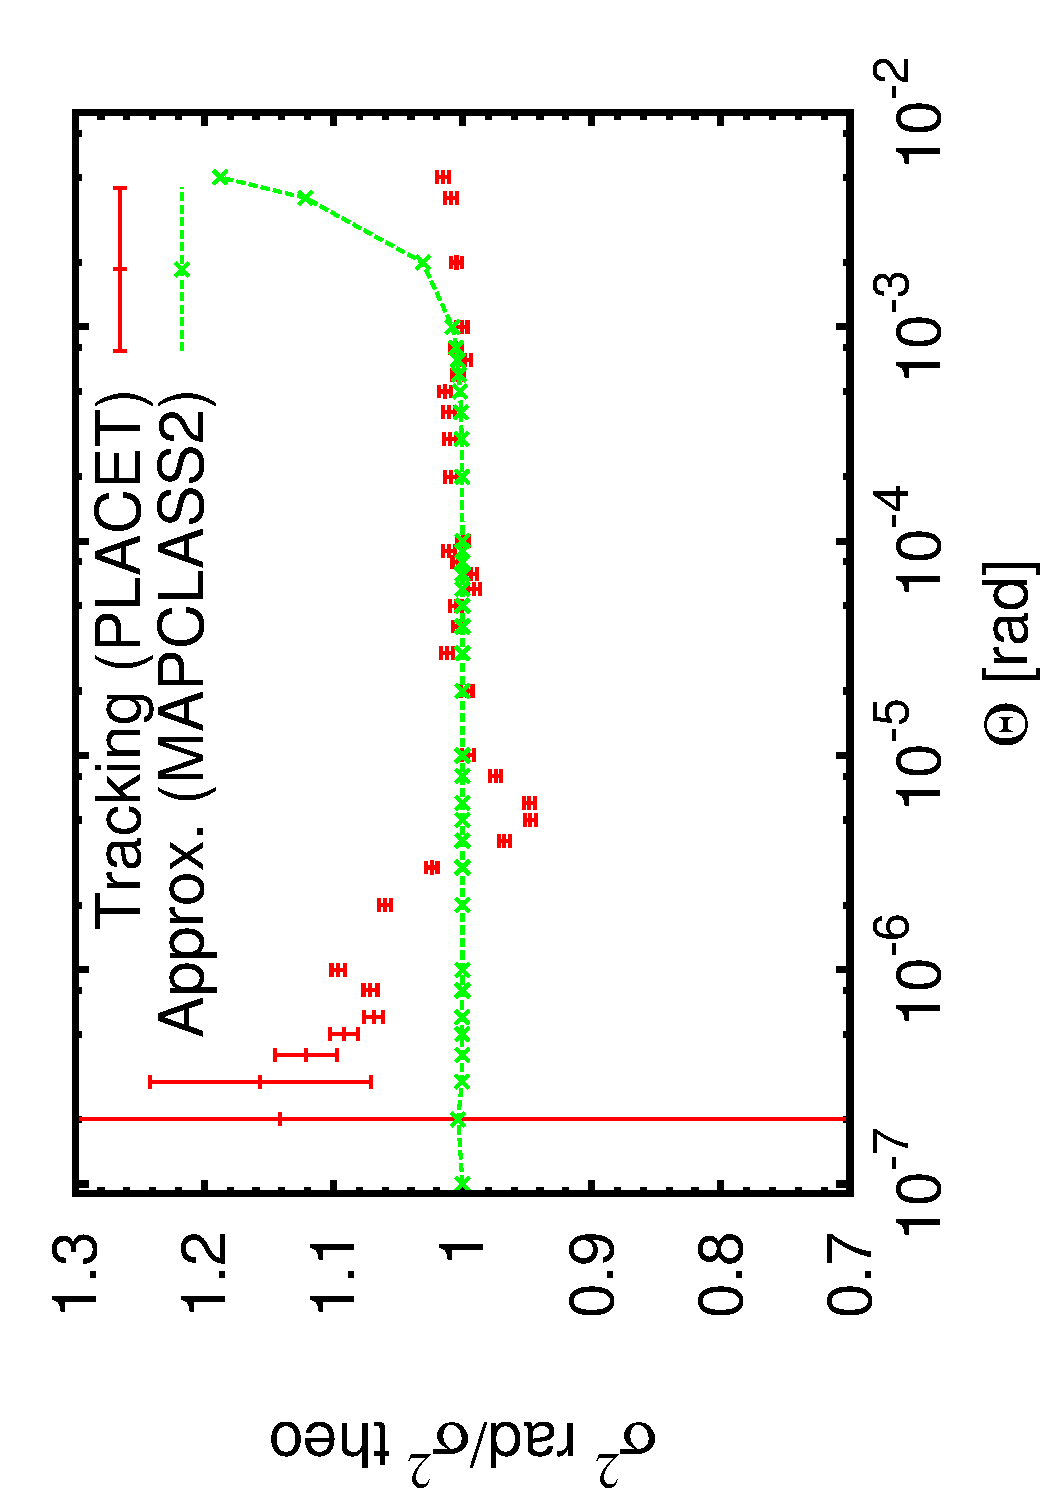
\includegraphics[scale=0.24,angle=-90]{sigma_angle_r6_twiss.pdf} \par
 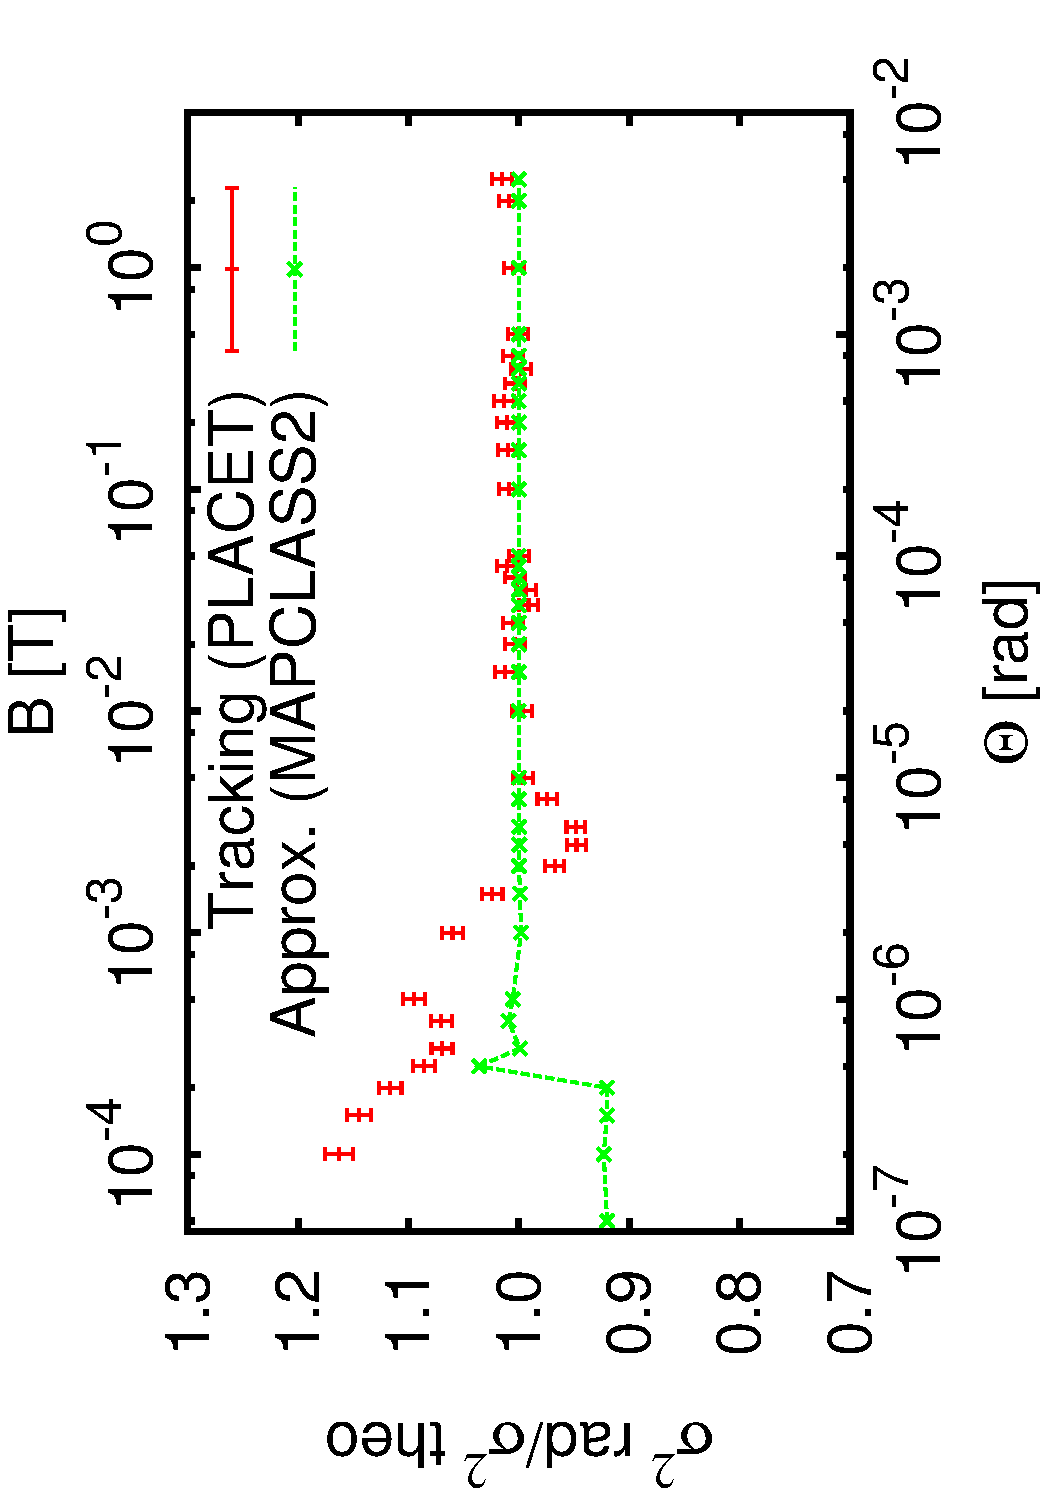
\includegraphics[scale=0.24,angle=-90]{sigma_angle_r06.pdf}
 \twisslogo
 \ptctwisslogo
\end{frame}


% \begin{frame}{Results (cont.)}
% Including a drift in front of the bending magnet.
% \begin{tabular}{p{3.5cm}p{10cm}}
% 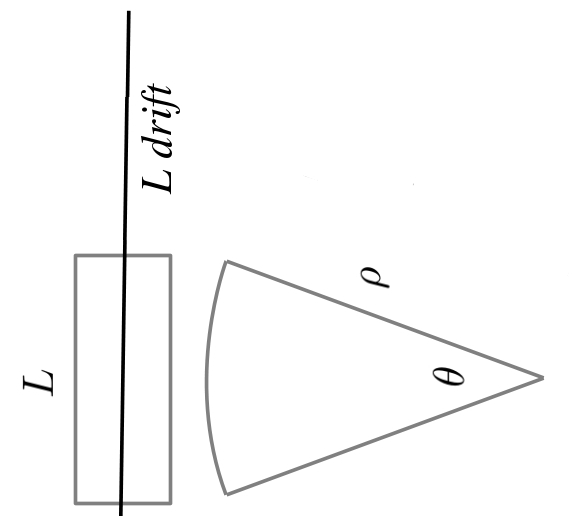
\includegraphics[angle=-90,scale=0.20]{Bend+drift2.jpg}&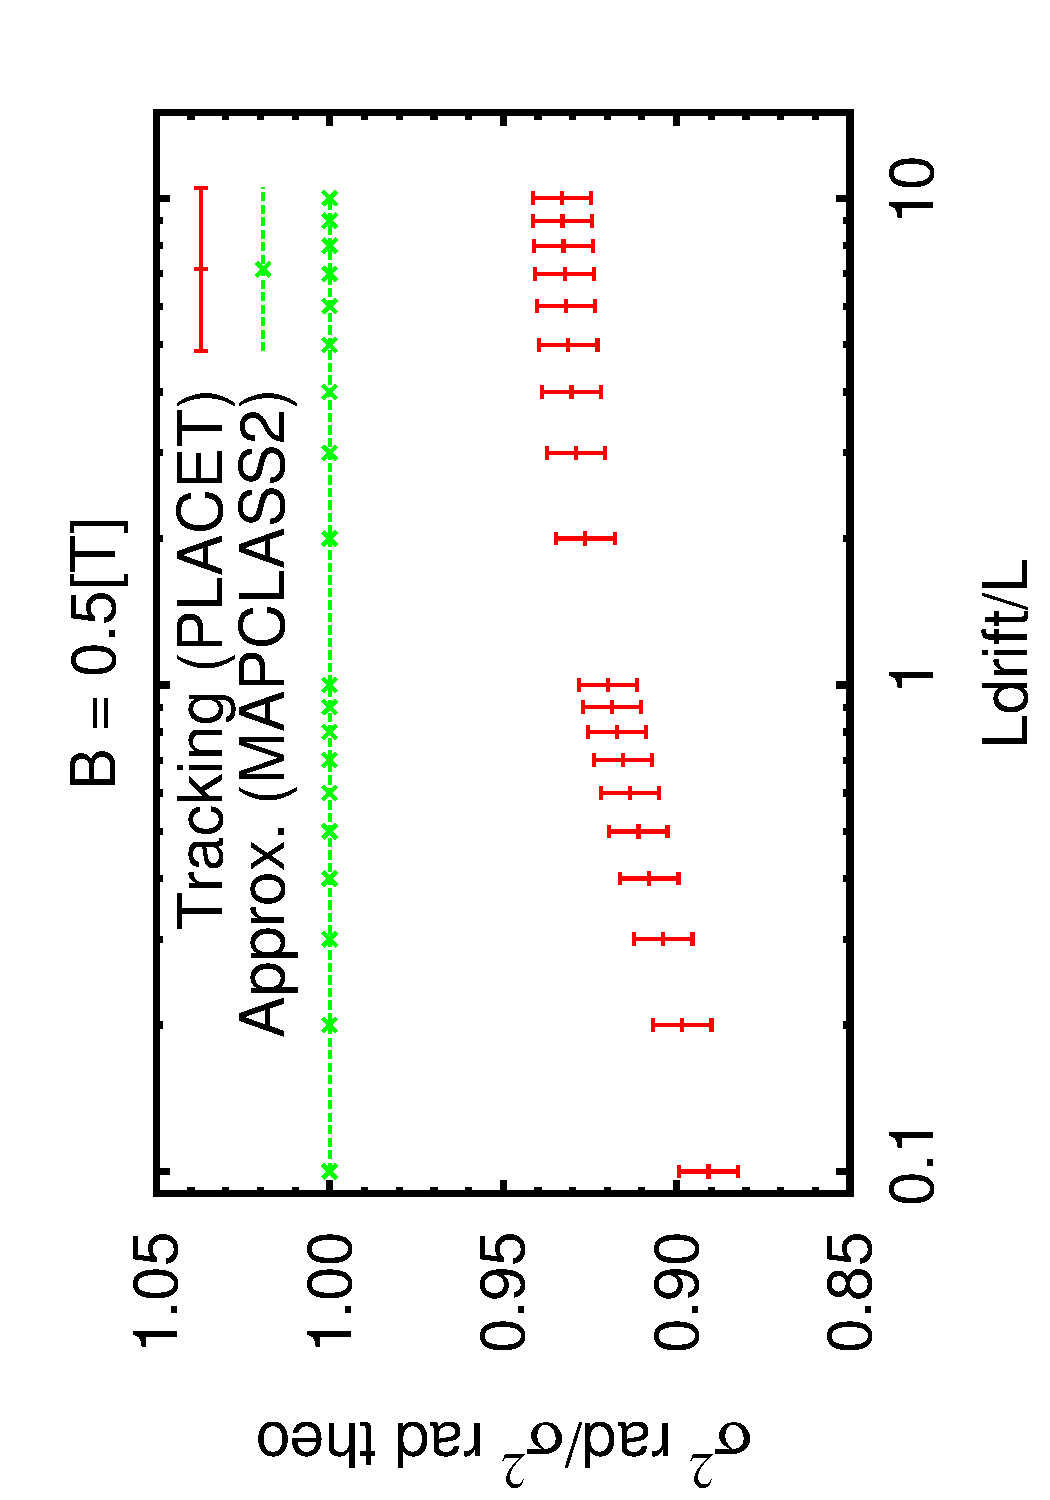
\includegraphics[angle=-90,scale=0.23]{sigma_Ldrift.pdf}%
% \end{tabular}
% 
%  In this case the radiation beamsize has been normalized to {\color{green}the approximated result}\par
% \textbf{Agreement between 80\% and 90\%}
% \end{frame}

% \section{Optimization Results and Conclusions}
% \subsection{Optimization}
% \begin{frame}{Optimization}
% The total length is fixed.
%  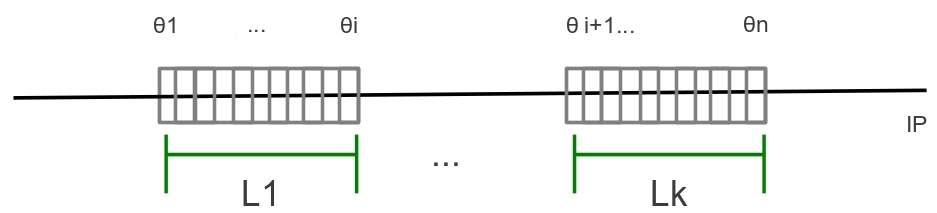
\includegraphics[width=10cm,height=3cm]{dipolesect.jpg}\par
% Total angle distribution will be changed to minimize ${\color{blue}\sigma_{rad}}$, under the following constraints:
% \begin{itemize}
%  \item $\eta_x(IP) = 0$
%  \item $\eta'_x(IP) = $constant value
% \end{itemize}
% \end{frame}
% \begin{frame}{Result}
% \begin{tabular}{lcc}
%  & $\sigma_{bef}$[nm]&$\sigma_{aft}$[nm]\\
% CLIC 3TeV & 46.28 & {\color{red}46.3}
% % CLIC 500GeV & 215.2 & -\\
% % ILC 500GeV & 477.2 & -\\
% \end{tabular}
% \begin{center}
%  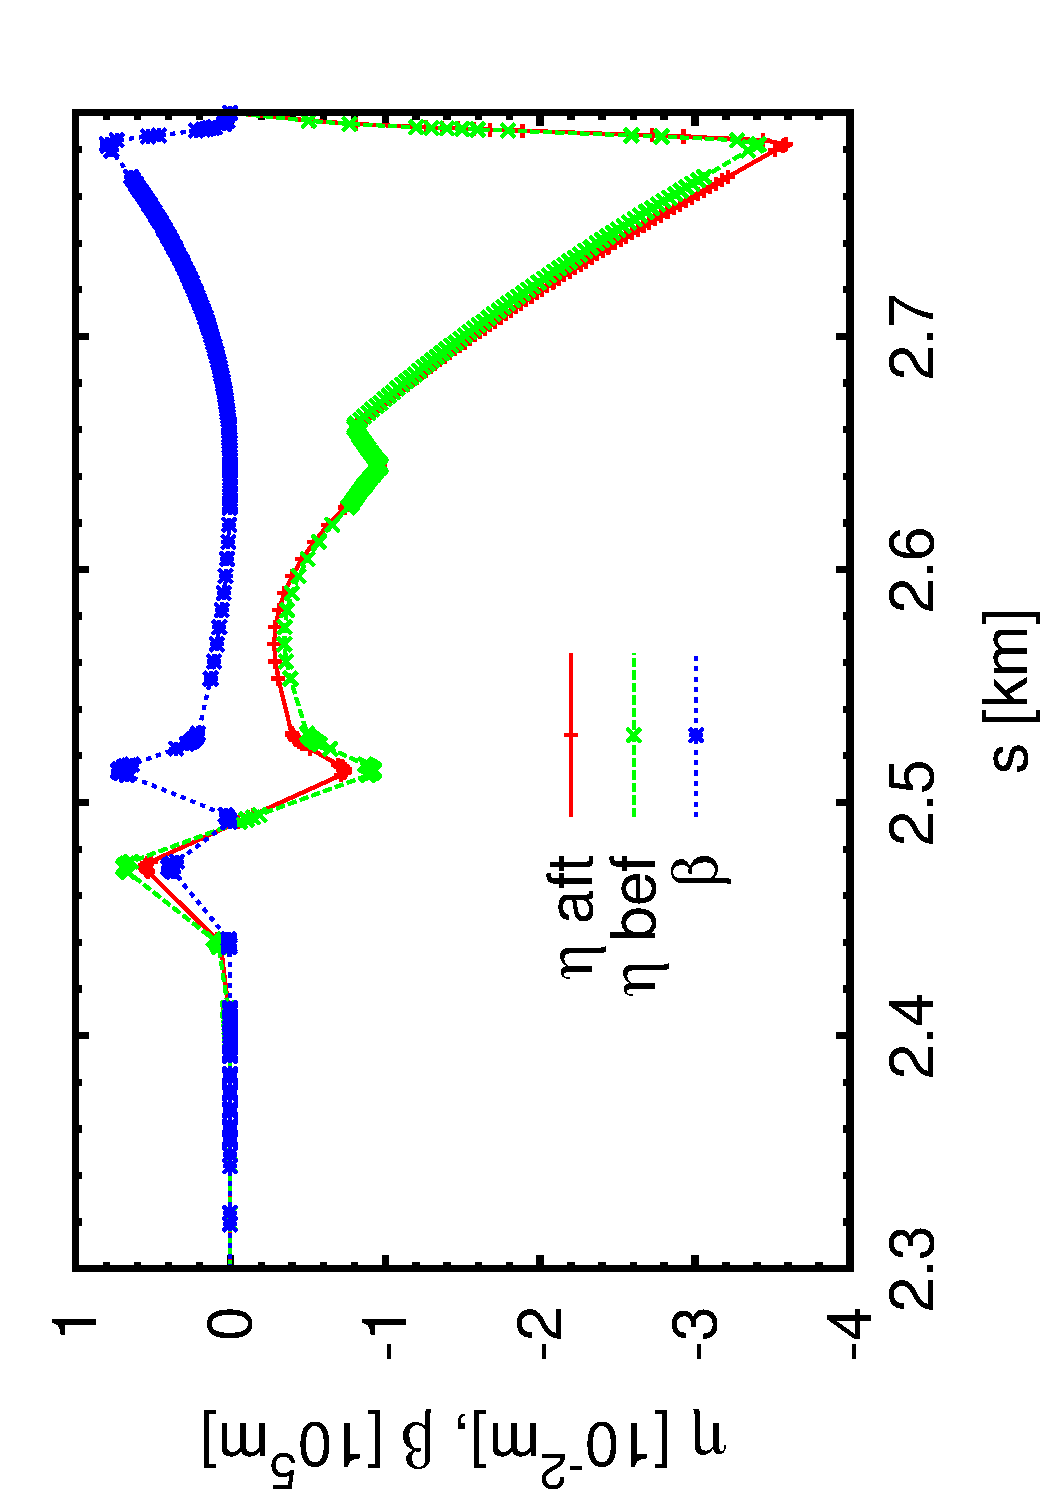
\includegraphics[scale=0.31,angle=-90]{eta_opt.pdf}
% \end{center}
% %  \begin{textblock}{1}(50,60)
% %   
% %  \end{textblock}
% %  \tiny
% %    
\includegraphics[height=1.6cm,keepaspectratio]{LAL.jpg}
% 
% 
%   
% \end{frame}
% % \begin{frame}
% %  However, beamsize is composed by
% %  \begin{equation*}
% %   \sigma^2 = \sigma_0^2 + \sigma_g^2+\sigma_\delta^2 +{\color{blue}	\sigma_{rad}^2}
% %  \end{equation*}
% % and, dispersion is used in the lattice to correct geometrical ($\sigma_g$) and chromatic ($\sigma_\delta$) aberrations (see \cite{Renier}).\par
% % It is required to include sextupoles in the optimization.
% % \end{frame}
% % \begin{frame}\hspace*{-1cm}
% %  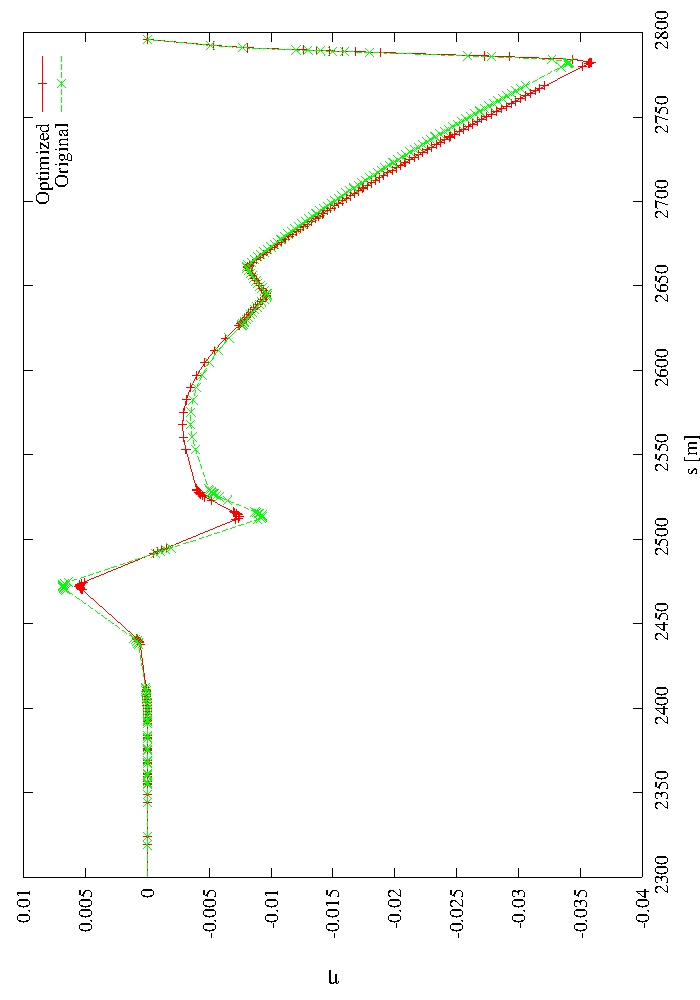
\includegraphics[width=7cm,height=12.7cm,angle=-90]{im02.png}
% %  \begin{textblock}{1}(50,180)
% %  \tiny
% % %    
\includegraphics[height=1.6cm,keepaspectratio]{LAL.jpg}
% % \begin{tabular}{lcc}
% %  & $\sigma$[nm] & ${\color{blue} \sigma^2_{bends}}[10^{-16}$m$^2$]\\
% % CLIC 3TeV & 46.3&5.54\\
% % CLIC 500GeV & 215.3&1.94\\
% % ILC 500GeV & 477.6&3.56\\
% % \end{tabular}
% % 
% %   \end{textblock}
% % \end{frame}

% \subsection{Conclusion}
\subsection{Low number of photons}
\begin{frame}{Low number of photons}
Average number of photons emitted is
\begin{align}
 \langle N\rangle&= \frac{1}{c} \int_0^L ds \int_0^\infty du\; n(u,s)\\
 &\approx C_1E\theta\qquad\qquad\qquad;C_1=20.61\text{[GeV]}^{-1}
\end{align}
\par
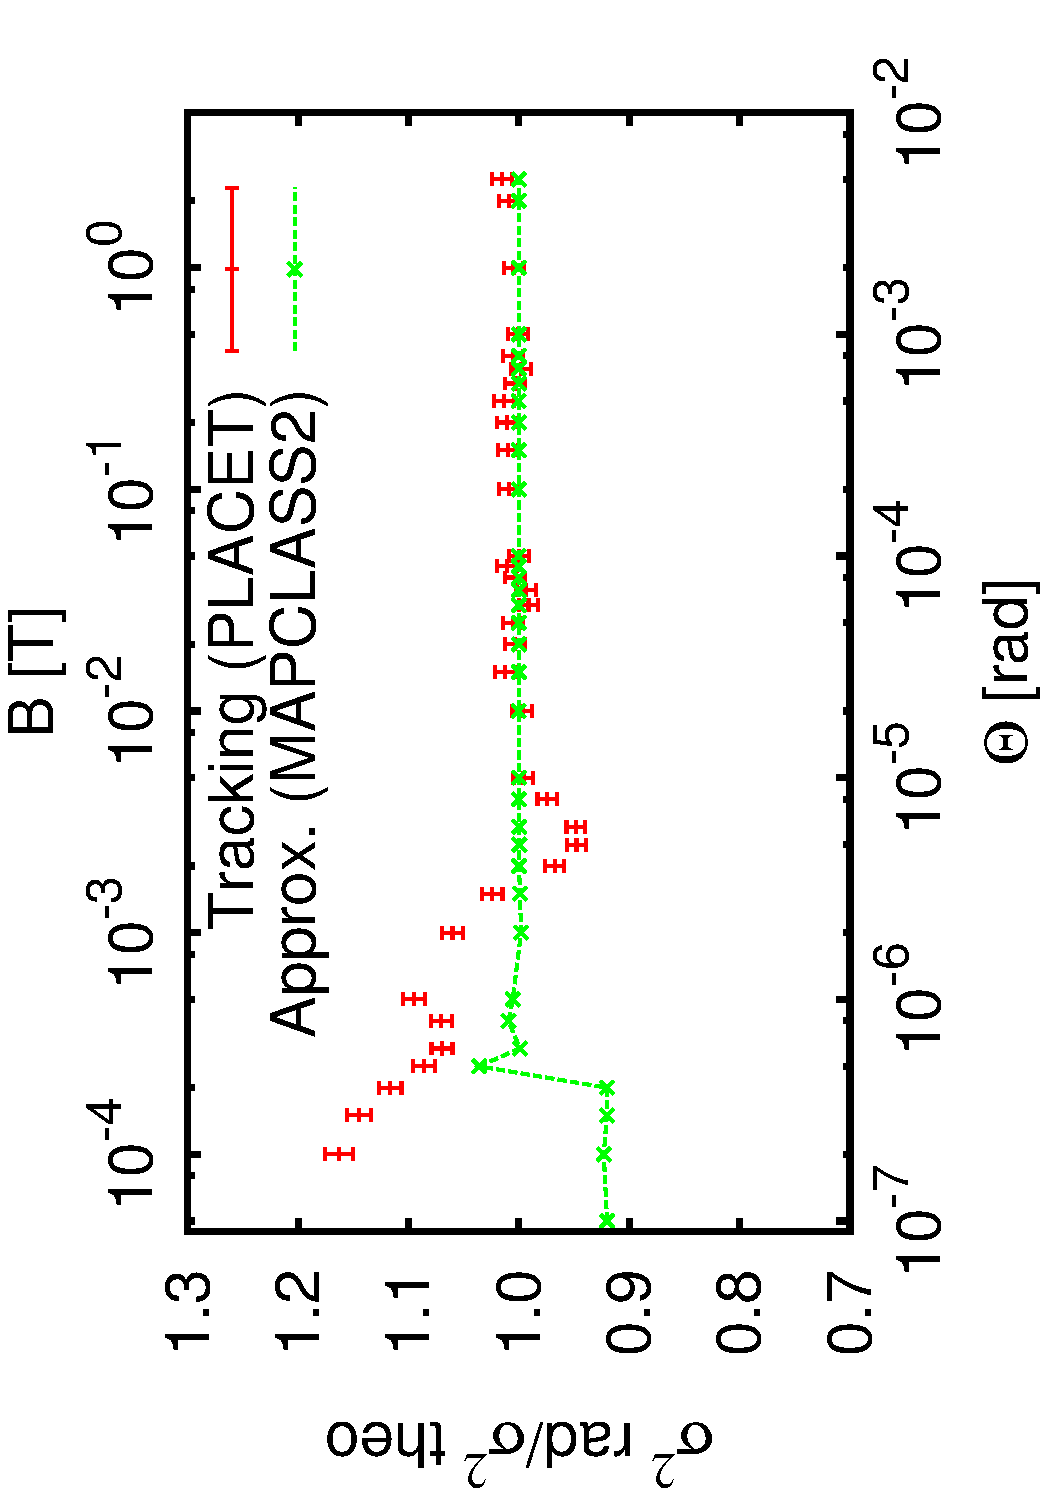
\includegraphics[scale=0.24,angle=-90]{sigma_angle_r06.pdf}
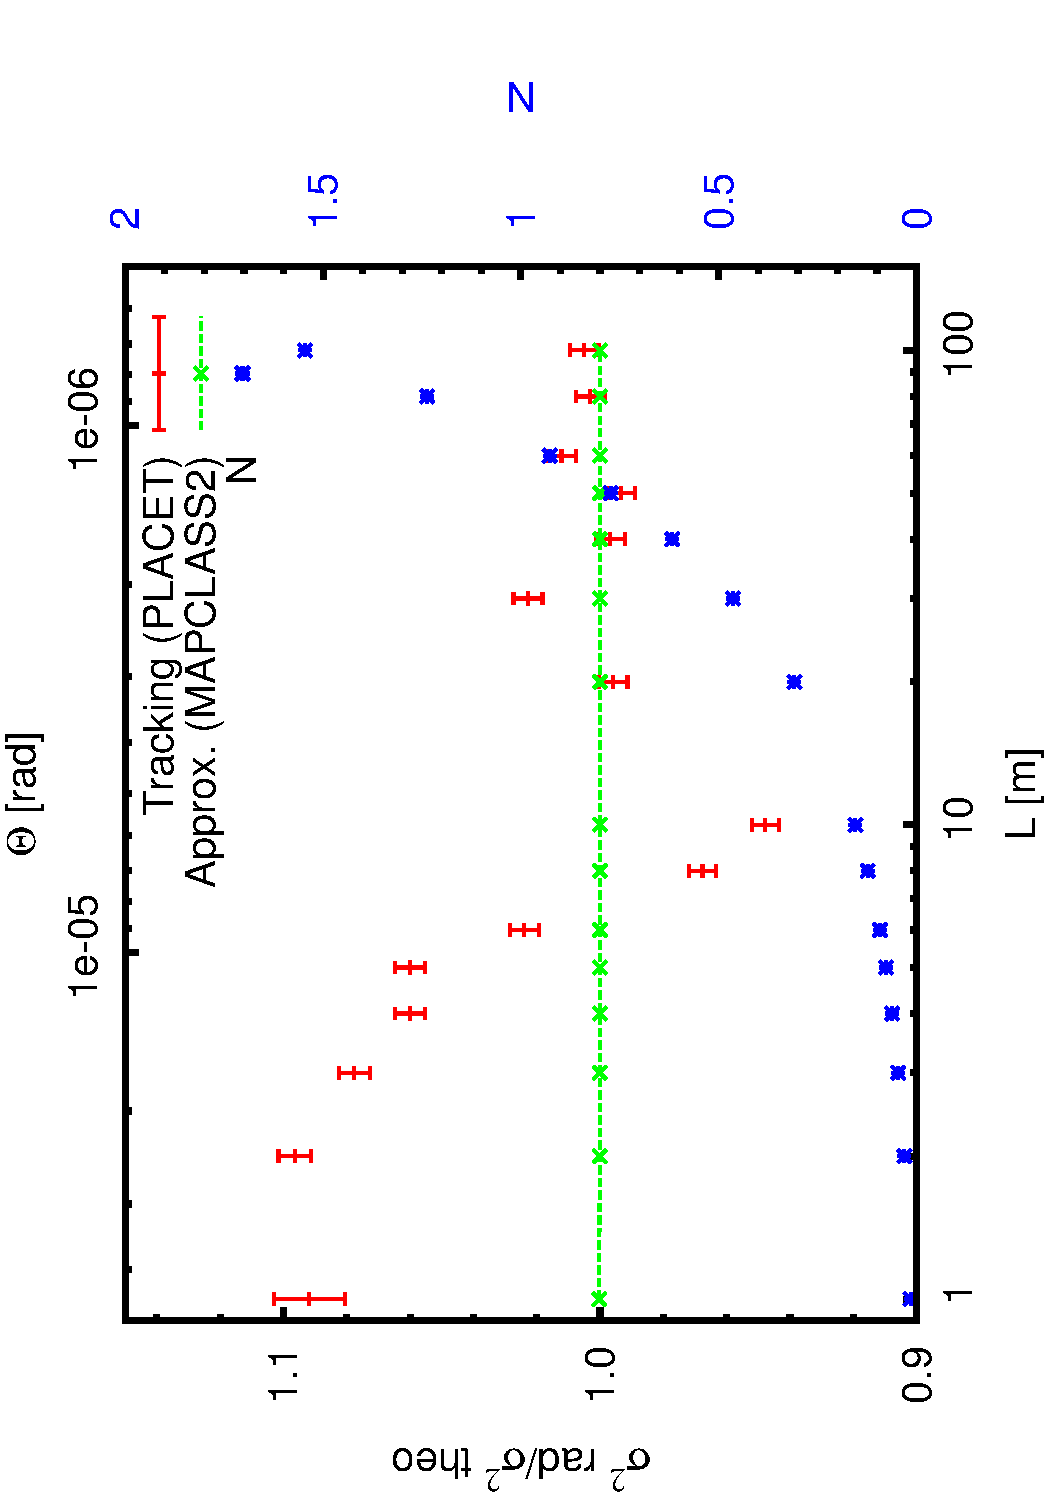
\includegraphics[scale=0.22,angle=-90]{sigma_Bfix5e-3T.pdf}

\end{frame}

\begin{frame}
%  \begin{array}{cc}
%  \hspace*{2.3cm}Default Synrad\hspace*{3.3cm}Flag ``-six\_dim 1''\par
 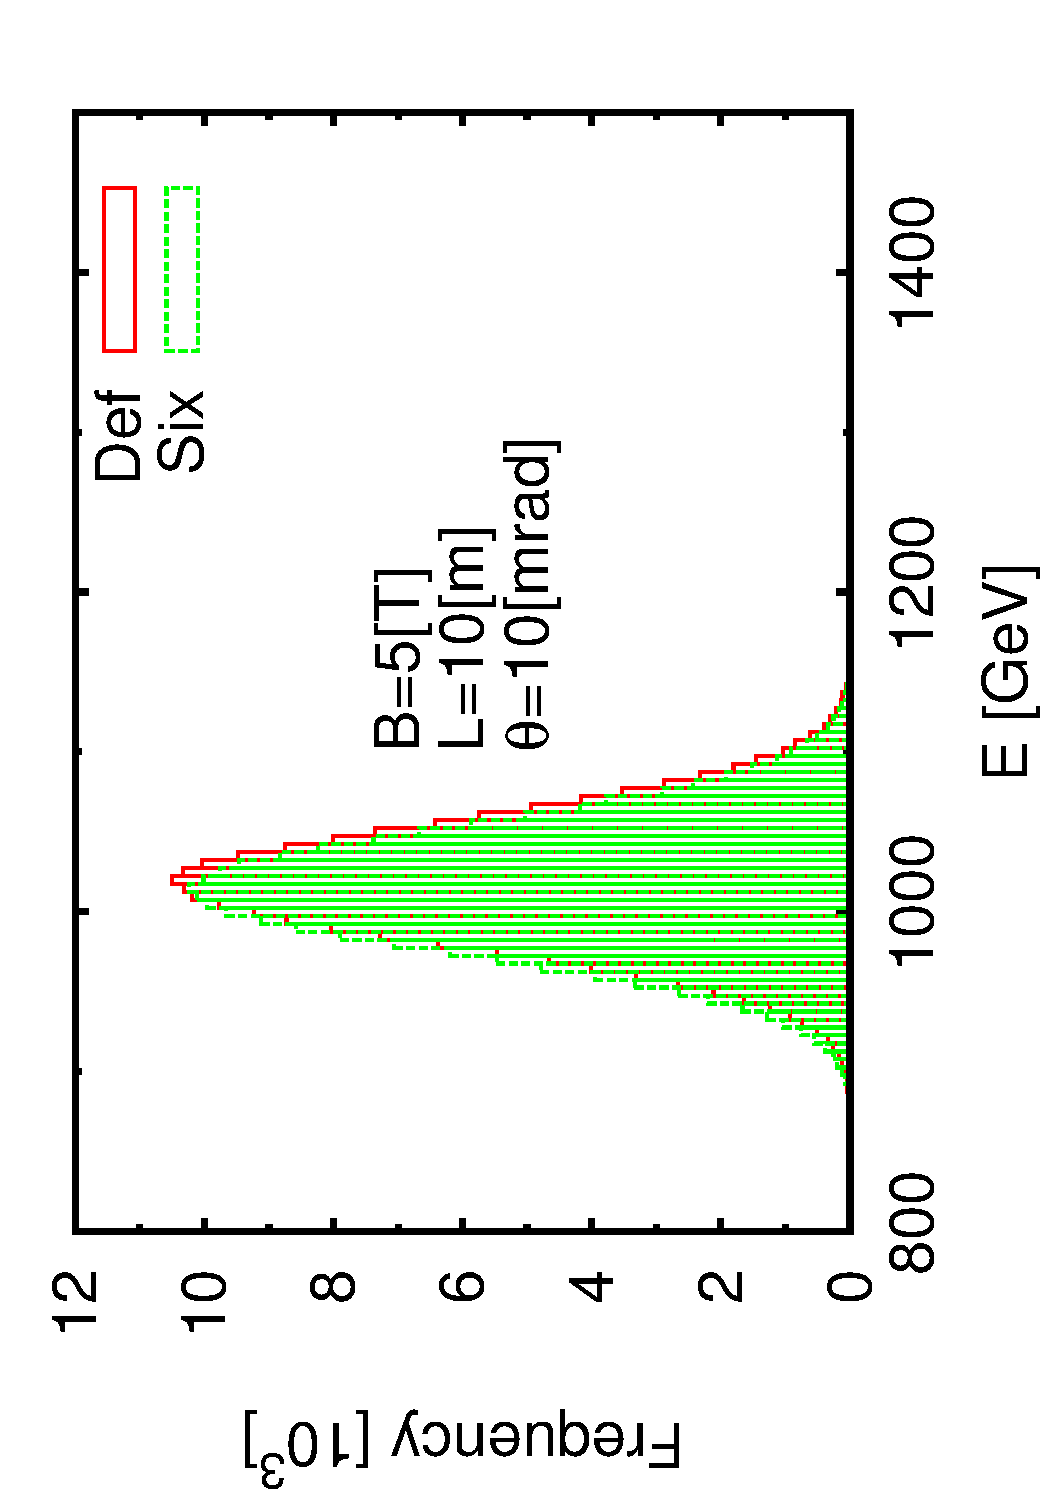
\includegraphics[scale=0.24,angle=-90]{histogram1e-2.pdf}
 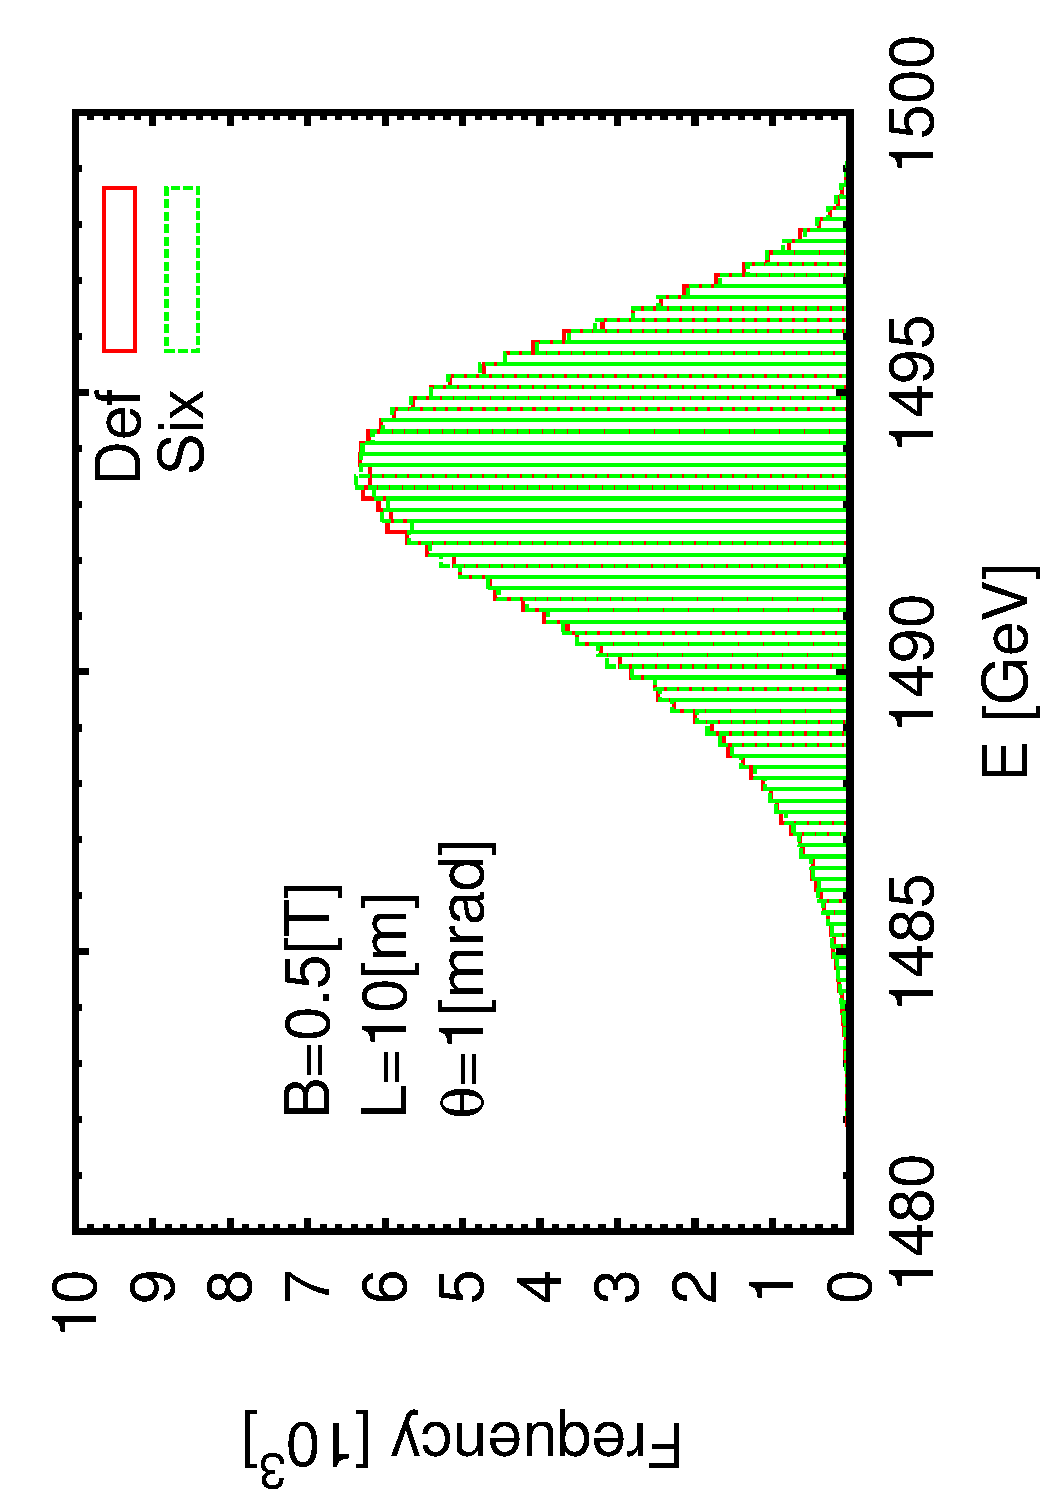
\includegraphics[scale=0.24,angle=-90]{histogram1e-3.pdf}\par
  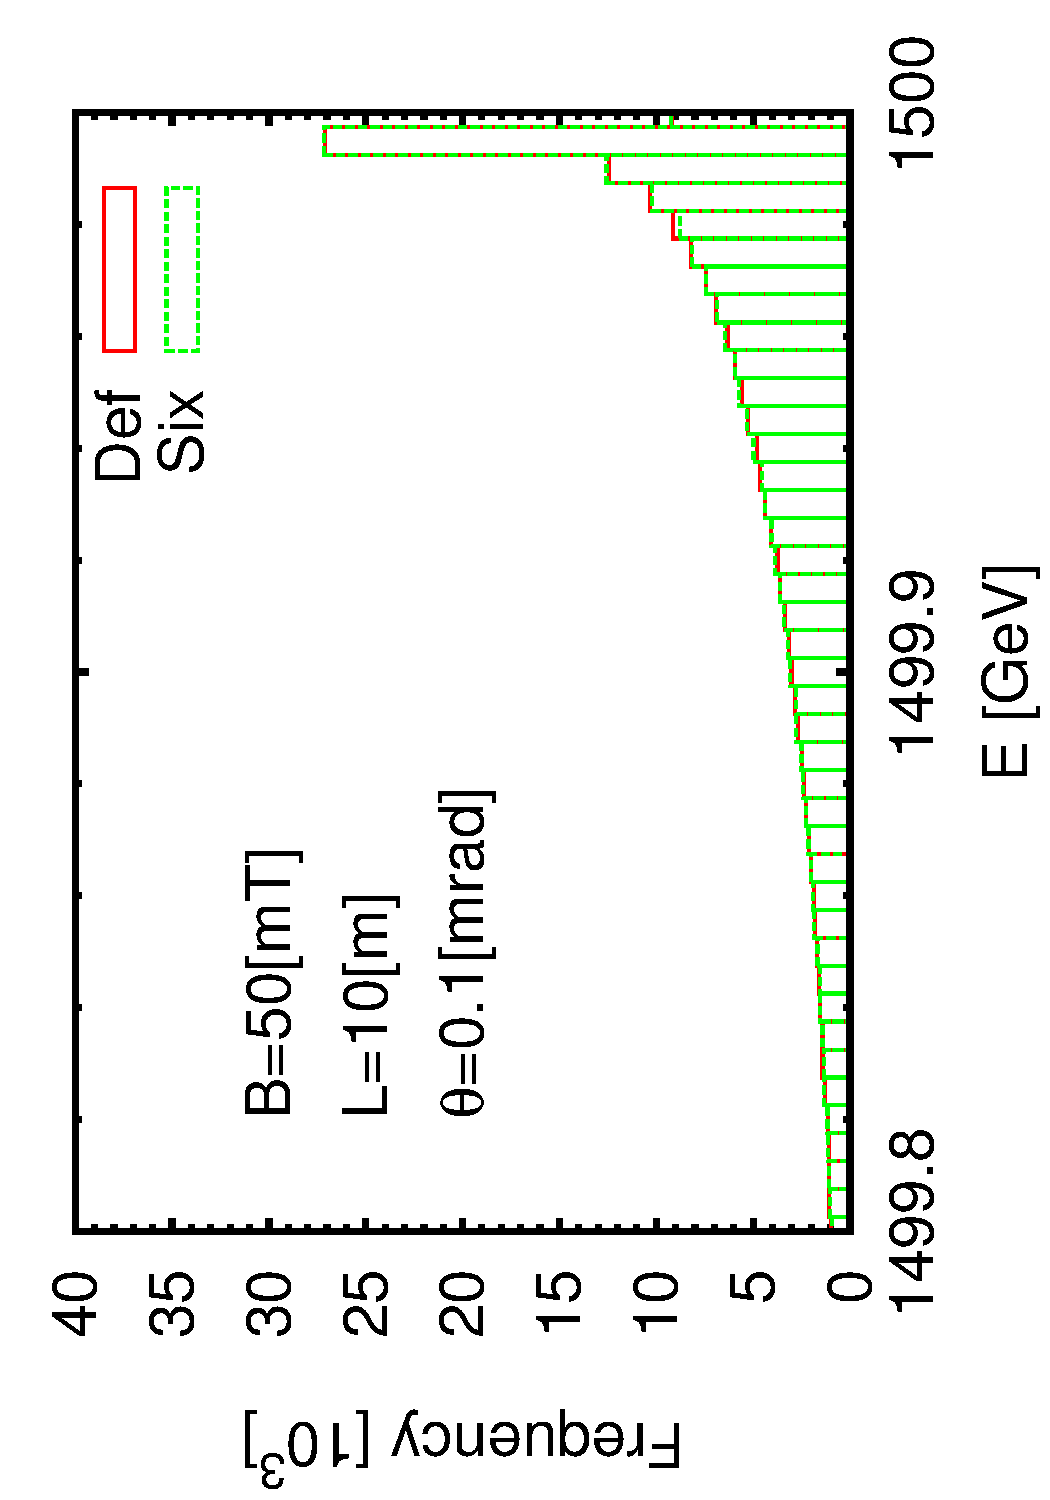
\includegraphics[scale=0.24,angle=-90]{histogram1e-4.pdf}
 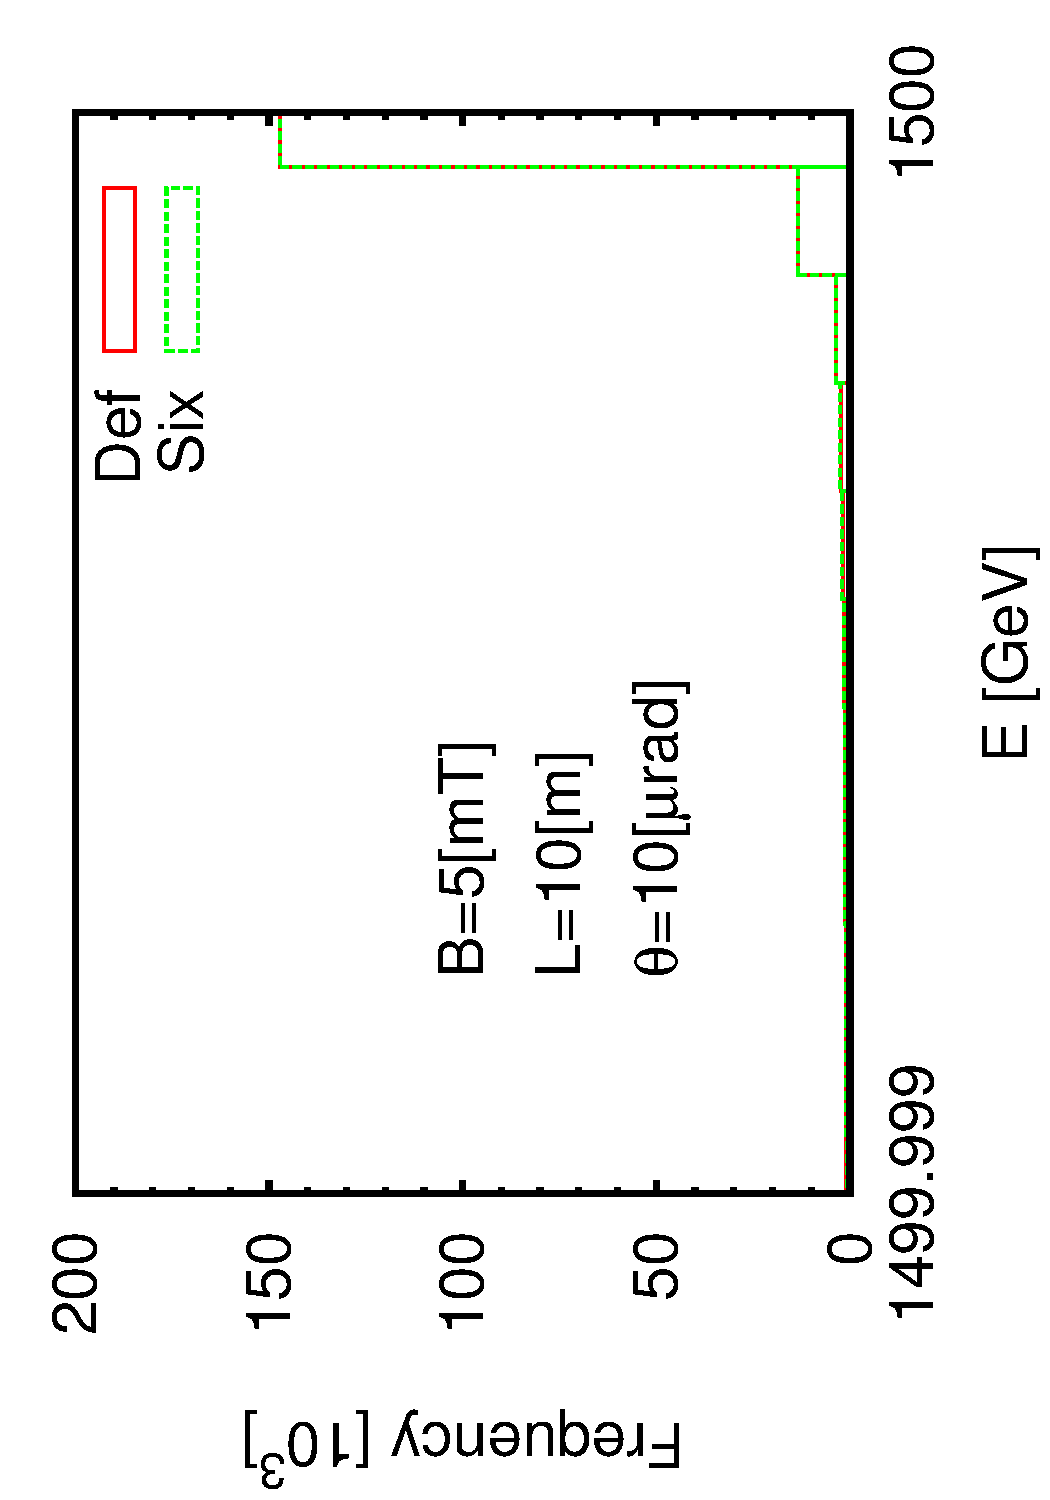
\includegraphics[scale=0.24,angle=-90]{histogram1e-5.pdf}\par
%  \end{array}

\end{frame}

\subsection{Conclusions}
\begin{frame}{Conclusions}
\begin{itemize}
 %\item The lattice was already optimized to balance between correction of aberrations and radiation effects. Differences in beamsizes are minimum.
 \item Mapclass2 agrees with theory, some care should be taken with twiss file.
 \item ``six\_dim'' in PLACET radiation model is more accurate than default radiation calculation. Both shows differences with theoretical model for bends causing low photon emission.
 \item Theoretical model for low photon emission stills in check.

%  \item 
%  \item Any region with large betas could be used to place bending magnets with minimum effect on radiation.
%  \item Next optimizations will include more parameters.
\end{itemize}

\end{frame}
% \subsection{Optimization}

\section*{References}
\begin{frame}{References}
 \begin{thebibliography}{6}
%  \bibitem{Oide} Oide, Katsunobu. Synchrotron-Radiation Limit on the Focusing of Electron Beams.	Phys. Rev. Lett. 61 – Issue 15, Oct, 1988. Pages 1713 – 1715.
 \bibitem{Sands} Sands, Matthew. Emittance growth from radiation fluctuations. SLAC/AP – 47. December, 1985.
 \bibitem{Renier} Renier, Ives. Implementation and validation of the linear collider final focus prototype : ATF2 at KEK (Japan). Doctoral Thesis, LAL10-91. June 2010.
 \end{thebibliography}
\end{frame}
\begin{frame}{Additional slides}
Dispersion function
\begin{equation*}
\begin{pmatrix}
 \eta(s_2)\\
 \eta'(s_2)\\
 1
\end{pmatrix}
=
\begin{pmatrix}
 C(s_1,s_2) & S(s_1,s_2)& R_{16}(s_1,s_2)\\
 C'(s_1,s_2) & S'(s_1,s_2) & R_{26}(s_1,s_2)\\
 0 & 0 &1
 
\end{pmatrix}
\begin{pmatrix}
 \eta(s_1)\\
 \eta'(s_1)\\
 1
\end{pmatrix}
\end{equation*}
PLACET error bars
\begin{align*}
 f&= \frac{x_{rad}^2-x_{norad}^2}{x^2_0}\\
 \delta f &= \frac{2}{\sqrt{N_{part}}}\frac{(x^2_{rad}+x^2_{norad})}{x_0^2}
\end{align*}
\end{frame}

\begin{frame}
Higher angle: most particles radiate.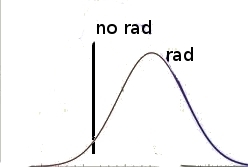
\includegraphics[scale=0.3]{gauss2.jpg} \par
Lower angle: some particles radiate, others don't.
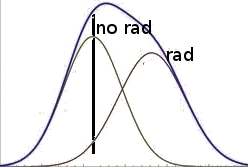
\includegraphics[scale=0.3]{gauss2a.jpg} 
\par

\begin{equation}
un(u) du \equiv P(u/\hbar)du/\hbar =  P(\omega)d\omega
\end{equation}

\end{frame}

\end{document}
